\documentclass[table]{beamer}
%[]中可以使用draft、handout、screen、transparency、trancompress、compress等参数

%指定beamer的模式与主题
\mode<presentation>
{
  \usetheme{Madrid}
%\usetheme{Boadilla}
%\usecolortheme{default}
%\usecolortheme{orchid}
%\usecolortheme{whale}
%\usefonttheme{professionalfonts}
}

%\usetheme{Madrid}
%这里还可以选择别的主题:Bergen, Boadilla, Madrid, AnnArbor, CambridgeUS, Pittsburgh, Rochester, Warsaw, ...
%有导航栏的Antibes, JuanLesPins, Montpellier, ...
%有内容的Berkeley, PaloAlto, Goettingen, Marburg, Hannover, ...
%有最小导航栏的Berlin, Ilmenau, Dresden, Darmstadt, Frankfurt, Singapore, Szeged, ...
%有章和节表单的Copenhagen, Luebeck, Malmoe, Warsaw, ...

%\usecolortheme{default}
%设置内部颜色主题(这些主题一般改变block里的颜色);这个主题一般选择动物来命名
%这里还可以选择别的颜色主题,如默认的和有特别目的的颜色主题default,structure,sidebartab,全颜色主题albatross,beetle,crane,dove,fly,seagull,wolverine,beaver

%\usecolortheme{orchid}
%设置外部颜色主题(这些主题一般改变title里的颜色);这个主题一般选择植物来命名
%这里还可以选择别的颜色主题,如默认的和有特别目的的颜色主题lily,orchid,rose

%\usecolortheme{whale}
%设置字体主题;这个主题一般选择海洋动物来命名
%这里还可以选择别的颜色主题,如默认的和有特别目的的颜色主题whale,seahorse,dolphin

%\usefonttheme{professionalfonts}
%类似的还可以定义structurebold,structuresmallcapsserif,professionalfonts

% 控制 beamer 的风格,可以根据自己的爱好修改
%\usepackage{beamerthemesplit} %使用 split 风格
%\usepackage{beamerthemeshadow} %使用 shadow 风格
%\usepackage[width=2cm,dark,tab]{beamerthemesidebar}

%插入音标
%\usepackage{tipa}
%\AtBeginDocument{
  %\renewcommand\textipa{\fontencoding{T3}\selectfont}
%}
%\AtBeginDocument{
  %\renewcommand\textipa[2][r]{{\fontfamily{cm#1}\tipaencoding #2}}
%}
%\renewenvironment{IPA}[1][r]
 %{\fontfamily{cm#1}\tipaencoding}
 %{}

% 设定英文字体
%\usepackage{fontspec}
% Fix bugs for fontspec in TeXLive2015
\ifdefined\suppressfontnotfounderror
  \expandafter\let\csname xetex_suppressfontnotfounderror:D\endcsname
    \suppressfontnotfounderror
\else
  \expandafter\let\csname xetex_suppressfontnotfounderror:D\endcsname
    \luatexsuppressfontnotfounderror
\fi
\usepackage[no-math]{fontspec}
\setmainfont{Times New Roman}
\setsansfont{Arial}
\setmonofont{Courier New}

% 设定中文字体
\usepackage[BoldFont,SlantFont,CJKchecksingle,CJKnumber]{xeCJK}
%\setCJKmainfont[BoldFont={Adobe Heiti Std},ItalicFont={Adobe Kaiti Std}]{Adobe Song Std}
\setCJKmainfont[BoldFont={Adobe Heiti Std},ItalicFont={Adobe Kaiti Std}]{WenQuanYi Micro Hei}
\setCJKsansfont{Adobe Heiti Std}
\setCJKmonofont{Adobe Fangsong Std}
\punctstyle{hangmobanjiao}

\defaultfontfeatures{Mapping=tex-text}
\usepackage{xunicode}
\usepackage{xltxtra}

\XeTeXlinebreaklocale "zh"
\XeTeXlinebreakskip = 0pt plus 1pt minus 0.1pt

\usepackage{setspace}
\usepackage{colortbl,xcolor}
\usepackage{hyperref}
%\hypersetup{xetex,bookmarksnumbered=true,bookmarksopen=true,pdfborder=1,breaklinks,colorlinks,linkcolor=blue,filecolor=black,urlcolor=cyan,citecolor=green}
\hypersetup{xetex,bookmarksnumbered=true,bookmarksopen=true,pdfborder=1,breaklinks,colorlinks,linkcolor=cyan,filecolor=black,urlcolor=blue,citecolor=green}

% 插入图片
\usepackage{graphicx}
\graphicspath{{figures/}}
% 图文混排
%\usepackage{picins}
\usepackage{floatflt}

% 可能用到的包
\usepackage{amsmath,amssymb}
%插入多媒体
%\usepackage{media9}
%\usepackage{movie15}
\usepackage{multimedia}
\usepackage{multicol}
\usepackage{multirow}

% 定义一些自选的模板,包括背景、图标、导航条和页脚等,修改要慎重
% 设置背景渐变由10%的红变成10%的结构颜色
%\beamertemplateshadingbackground{red!10}{structure!10}
%\beamertemplatesolidbackgroundcolor{white!90!blue}
% 使所有隐藏的文本完全透明、动态,而且动态的范围很小
\beamertemplatetransparentcovereddynamic
% 使itemize环境中变成小球,这是一种视觉效果
\beamertemplateballitem
% 为所有已编号的部分设置一个章节目录,并且编号显示成小球
\beamertemplatenumberedballsectiontoc
% 将每一页的要素的要素名设成加粗字体
\beamertemplateboldpartpage

% item逐步显示时,使已经出现的item、正在显示的item、将要出现的item呈现不同颜色
\def\hilite<#1>{
 \temporal<#1>{\color{gray}}{\color{blue}}
    {\color{blue!25}}
}

\renewcommand{\today}{\number\year 年 \number\month 月 \number\day 日}

%五角星
\usepackage{MnSymbol}

%去除图表标题中的figure等
\usepackage{caption}
\captionsetup{labelformat=empty,labelsep=none}

\usepackage{tabu}
\usepackage{multirow}
%表格自动换行
\usepackage{tabularx} 

% 千分号
%\usepackage{textcomp}

%罗马数字
\makeatletter
\newcommand{\rmnum}[1]{\romannumeral #1}
\newcommand{\Rmnum}[1]{\expandafter\@slowromancap\romannumeral #1@}
\makeatother

%分栏
\usepackage{multicol}

%\usepackage{enumitem}
%\usepackage{enumerate}

%键盘
\usepackage{keystroke}

%心形
\usepackage{fdsymbol}

%插入源代码
\usepackage{listings}
\lstset{
  language=perl,                  % 程序语言名称:TeX, Perl, R, sh, bash, Awk
  basicstyle=\normalsize\tt,      %\tt指monospace字体族,程序源代码使用此族字体表示更加美观
  numbers=left,                   % 行号位置(左侧)
  numberstyle=\small,             % 行号字体的字号
  stepnumber=1,                   % 行号的显示步长
  numbersep=5pt,                  % 行号与代码间距
  backgroundcolor=\color{white},  % 背景色;需要 \usepackage{color}
  showspaces=false,               % 不显示空格
  showstringspaces=false,         % 不显示代码字符串中的空格标记
  showtabs=false,                 % 不显示 TAB
  tabsize=4, 
  frame=shadowbox,                % 把代码用带有阴影的框圈起来
  captionpos=b,                   % 标题位置
  breaklines=true,                % 对过长的代码自动断行
  breakatwhitespace=false,        % 断行只在空格处
  extendedchars=false,            % 解决代码跨页时,章节标题,页眉等汉字不显示的问题
  %escapeinside={\%*}{*},         % 跳脱字符,添加注释,暂时离开 listings 
  %escapeinside=``,
  commentstyle=\color{red!50!green!50!blue!50}\tt,  %浅灰色的注释
  rulesepcolor=\color{red!20!green!20!blue!20},     %代码块边框为淡青色
  keywordstyle=\color{blue!70}\bfseries\tt,         %代码关键字的颜色为蓝色,粗体
  identifierstyle=\tt,
  stringstyle=\tt,                % 代码字符串的特殊格式
  keepspaces=true,
  breakindent=1em,
  %breakindent=22pt,
  %breakindent=4em,
  breakautoindent=true,
  flexiblecolumns=true,
  aboveskip=1em,                  %代码块边框
  xleftmargin=2em,
  xrightmargin=2em
}

%\setbeamercolor{alerted text}{fg=magenta}
\setbeamercolor{bgcolor}{fg=yellow,bg=cyan}
%\setbeamercolor{itemize/enumerate body}{fg=green}

\begin{document}

%\includeonlyframes{current}

\logo{\includegraphics[height=0.08\textwidth]{tijmu.png}}

% 在每个Section前都会加入的Frame
\AtBeginSection[]
{
  \begin{frame}<beamer>
    %\frametitle{Outline}
    \frametitle{教学提纲}
    \setcounter{tocdepth}{3}
    \begin{multicols}{2}
      \tableofcontents[currentsection,currentsubsection]
      %\tableofcontents[currentsection]
    \end{multicols}
  \end{frame}
}
% 在每个Subsection前都会加入的Frame
\AtBeginSubsection[]
{
  \begin{frame}<beamer>
%%\begin{frame}<handout:0>
%% handout:0 表示只在手稿中出现
    \frametitle{教学提纲}
    \setcounter{tocdepth}{3}
    \begin{multicols}{2}
    \tableofcontents[currentsection,currentsubsection]
    \end{multicols}
%% 显示在目录中加亮的当前章节
  \end{frame}
}

% 为当前幻灯片设置背景
%{
%\usebackgroundtemplate{
%\vbox to \paperheight{\vfil\hbox to
%\paperwidth{\hfil\includegraphics[width=2in]{tijmu_charcoal.png}\hfil}\vfil}
%}
\begin{frame}[plain]
  \begin{center}
    {\Huge 分子生物计算\\}
    {\huge \textit{(Perl语言编程)}\\}
    \vspace{1cm}
    {\LARGE 天津医科大学\\}
    %\vspace{0.2cm}
    {\LARGE 生物医学工程与技术学院\\}
    \vspace{1cm}
    {\large 2019-2020学年上学期(秋)\\ 2017级生信班}
  \end{center}
\end{frame}
%}



\title[基序和循环]{第五章\quad 基序和循环}
\author[Yixf]{伊现富(Yi Xianfu)}
\institute[TIJMU]{天津医科大学(TIJMU)\\ 生物医学工程与技术学院}
\date{2016年11月}

\input{snippet/beamer_toc.tex}


\section{引言}
\begin{frame}
  \frametitle{基序和循环 | 引言 | 已经学习}
  \begin{block}{Perl语言基础}
    \begin{itemize}
      \item 标量变量和数组变量
      \item 字符串操作(替换、翻译等)
      \item 从文件中读取数据
    \end{itemize}
  \end{block}
  \pause
  \begin{block}{DNA和蛋白质生物序列数据的处理}
    \begin{itemize}
      \item 拼接DNA片段
      \item 把DNA转录成RNA
      \item 获取反向互补序列
      \item 从文件中读取序列
    \end{itemize}
  \end{block}
\end{frame}
\begin{frame}
  \frametitle{基序和循环 | 引言 | 即将学习}
  \begin{block}{Perl语言基础}
    \begin{itemize}
      \item 根据条件测试的结果采取不同的行动
      \item 使用循环
      \item 通过键盘与用户进行交互
      \item 使用基本的正则表达式
      \item 操作字符串和数组
      \item 把处理结果写入文件
    \end{itemize}
  \end{block}
  \pause
  \begin{block}{DNA和蛋白质序列数据的处理}
    \begin{itemize}
      \item 使用循环读取文件中的序列数据
      \item 查找蛋白质序列中的基序
      \item 计算核苷酸频率
    \end{itemize}
  \end{block}
\end{frame}

\section{流程控制}
\begin{frame}
  \frametitle{基序和循环 | 流程控制 | 简介}
  \begin{block}{定义}
    控制流程(也称为流程控制,flow control)是电脑运算领域的用语,意指在程序运行时,个别的指令(或是陈述、子程序)运行或求值的顺序。
  \end{block}
  \pause
  \begin{block}{指令}
    不同的编程语言所提供的流程控制指令也会随之不同,但一般可以分为以下几种:
    \begin{itemize}
      \item 继续运行位于不同位置的一段指令(无条件分支指令)。
      \item 若特定条件成立时,运行一段指令,例如C语言的switch指令,是一种有条件分支指令。
      \item 运行一段指令若干次,直到特定条件成立为止,例如C语言的for指令,仍然可视为一种有条件分支指令。
      \item 运行位于不同位置的一段指令,但完成后会继续运行原来要运行的指令,包括子程序、协程(coroutine)及延续性(continuation)。
      \item 停止程序,不运行任何指令(无条件的终止)。
    \end{itemize}
  \end{block}
\end{frame}

\begin{frame}
  \frametitle{基序和循环 | 流程控制 | 分类}
  \begin{block}{默认}
    除非明确指明不按顺序执行,否则程序将从最顶端的第一个语句开始,顺序执行到最底端的最后一个语句。
  \end{block}
  \pause
  \begin{block}{\alert{分类}}
    \begin{itemize}
      \item 条件判断:只在条件测试成功的前提下执行相应的语句,否则直接跳过这些语句
      \item 循环:一直重复语句,直到相应的测试失败为止
    \end{itemize}
  \end{block}
\end{frame}

\subsection{条件判断}
\begin{frame}
  \frametitle{基序和循环 | 流程控制 | 条件判断}
  \begin{block}{\alert{Perl中的实现}}
    \begin{itemize}
      \item if
      \item if-else
      \item unless
    \end{itemize}
  \end{block}
  \pause
  \begin{block}{工作原理}
    \begin{itemize}
      \item 条件测试的结果为真(true)或者为假(false)
      \item 如果测试结果为真,后面的语句就会被执行
      \item 如果测试结果为假,后面的语句就不会执行,直接被跳过
    \end{itemize}
  \end{block}
\end{frame}

\begin{frame}[fragile]
  \frametitle{基序和循环 | 流程控制 | 条件判断 | \alert{if} | 真}
\begin{lstlisting}
# =表示赋值,==表示数字相等
if( 1 == 1 ) {
  print "1 equals 1\n\n";
}

if( 1 ) {
  print "1 evaluates to true\n\n";
}
\end{lstlisting}
\end{frame}

\begin{frame}[fragile]
  \frametitle{基序和循环 | 流程控制 | 条件判断 | \alert{if} | 假}
\begin{lstlisting}
if( 1 == 0 ) {
  print "1 equals 0\n\n";
}

if( 0 ) {
  print "0 evaluates to true\n\n";
}
\end{lstlisting}
\end{frame}

\begin{frame}[fragile]
  \frametitle{基序和循环 | 流程控制 | 条件判断 | if | \alert{简写}}
\begin{lstlisting}
# 两种写法完全等价
# 比较“标准”,易读易懂
if( 1 == 1 ) {
  print "1 equals 1\n\n";
}

# 更加简洁
print "1 equals 1\n\n" if (1 == 1);

# 类比自然语言(英语)
# If you build it, they will come.
# They will come if you build it.
\end{lstlisting}
\end{frame}
    
\begin{frame}[fragile]
  \frametitle{基序和循环 | 流程控制 | 条件判断 | \alert{if-else} | 真}
\begin{lstlisting}
if( 1 == 1 ) {
  print "1 equals 1\n\n";
} else {
  print "1 does not equal 1\n\n";
}

# 1 equals 1
\end{lstlisting}
\end{frame}

\begin{frame}[fragile]
  \frametitle{基序和循环 | 流程控制 | 条件判断 | \alert{if-else} | 假}
\begin{lstlisting}
if( 1 == 0 ) {
  print "1 equals 0\n\n";
} else {
  print "1 does not equal 0\n\n";
}

# 1 does not equal 0
\end{lstlisting}
\end{frame}

\begin{frame}[fragile]
  \frametitle{基序和循环 | 流程控制 | 条件判断 | \alert{unless}}
  \begin{block}{unless}
    \begin{itemize}
      \item unless和if完全相反
      \item 如果测试结果为真,语句会直接被跳过而不执行
      \item 如果测试结果为假,相应的语句会被执行
    \end{itemize}
  \end{block}
  \pause
\begin{lstlisting}
unless( 1 == 0 ) {
  print "1 does not equal 0\n\n";
}
# 1 does not equal 0

# 类比自然语言
# Unless you study Russian literature, you are ignorant of Chekov.
# 除非下课铃响了,否则我们不会下课。
\end{lstlisting}
\end{frame}

\begin{frame}[fragile]
  \frametitle{基序和循环 | 流程控制 | 条件判断 | unless vs. if}
\begin{lstlisting}
unless ( 1 == 0 ) {
  print "1 does not equal 0\n\n";
}
# 1 does not equal 0

if ( 1 != 0 ) {
  print "1 does not equal 0\n\n";
}
# 1 does not equal 0

if ( !(1 == 0) ) {
  print "1 does not equal 0\n\n";
}
# 1 does not equal 0
\end{lstlisting}
\end{frame}

\begin{frame}[fragile]
  \frametitle{基序和循环 | 流程控制 | 条件判断 | \alert{补充说明}}
  \begin{block}{条件测试}
    \begin{itemize}
      \item 数字比较:==, !=, <, >, <=, >=
      \item 字符串比较:eq, ne, lt, gt, le, ge
      \item 文件测试:-e, -s, -z, -f, -d, -l, -r, -w, -x, ...
      \item 变量测试:真(True),假(False)
    \end{itemize}
  \end{block}
\end{frame}

\begin{frame}[fragile]
  \frametitle{基序和循环 | 流程控制 | 条件判断 | 补充说明}
  \begin{block}{说谎者悖论}
    \begin{block}{}
      这个语句为假。
    \end{block}
    \begin{block}{}
      这个语句不为真。
    \end{block}
    \begin{block}{}
      这个语句只为假。
    \end{block}
    \begin{block}{}
    下个语句为真。\\
    上个语句为假。
    \end{block}
    \begin{block}{}
    第二个语句为假。\\
    第三个语句为假。\\
    第一个语句为假。
    \end{block}
  \end{block}
\end{frame}

\begin{frame}[fragile]
  \frametitle{基序和循环 | 流程控制 | 条件判断 | \alert{补充说明}}
  \begin{block}{真 vs. 假}
    \begin{itemize}
      \item 真假判定
       	\begin{itemize}
	        \item 如果是数字:0(0, 0.0, -0.0, ……)为假,其他所有数字都为真
          \item 如果是字符串:空字符串(用 \verb|""|或 \verb|''|表示)为假,其他所有字符串都为真【参看下一条目】
          \item 注意:字符串 \verb|'0'|或 \verb|"0"|(和数字0是同一个标量值)是唯一被当成假的非空字符串
	        \item 如果既不是数字也不是字符串,先转换成数字或字符串再行判断
        \end{itemize}
      \item 补充说明
       	\begin{itemize}
          \item \verb|""|, \verb|''|(空字符串) vs. \verb|" "|, \verb|' '|(空白/格字符串)
          \item 没有借阅证 vs. 有借阅证但没有借阅记录
        \end{itemize}
    \end{itemize}
  \end{block}
\end{frame}

\begin{frame}
  \frametitle{基序和循环 | 流程控制 | 条件判断 | 补充说明}
  \begin{block}{括号成对}
    \begin{itemize}
	\item (小、中、大、尖)括号成对是最普遍的编程特性
	\item 左右括号的数目相等且都出现在正确的位置
	\item 括号不配对或者没有在正确的位置是非常常见的语法错误
	\item 保证括号配对的方法:
	  \begin{itemize}
	    \item 每行/块代码做的事情不要太多
	    \item 使用缩进使代码块明显一些
	    \item 使用专用的文本编辑器(Vim中的\%)
	    \item 对代码进行格式化(perltidy)
	  \end{itemize}
    \end{itemize}
  \end{block}
\end{frame}

\begin{frame}[fragile]
  \frametitle{基序和循环 | 流程控制 | 条件判断 | \alert{if-elsif-else}}
\begin{lstlisting}
#!/usr/bin/perl -w

$word = 'MNIDDKL';

if($word eq 'QSTVSGE') {
  print "QSTVSGE\n";
} elsif($word eq 'MRQQDMISHDEL') {
  print "MRQQDMISHDEL\n";
} elsif ( $word eq 'MNIDDKL'  ) {
  print "MNIDDKL--the magic word!\n";
} else {
  print "Is \"$word\" a peptide? This program is not sure.\n";
}

exit;
\end{lstlisting}
\end{frame}

\subsection{循环}
\begin{frame}
  \frametitle{基序和循环 | 流程控制 | 循环}
  \begin{block}{\alert{Perl中的实现}}
    \begin{itemize}
      \item while
      \item for
      \item foreach
      \item until
    \end{itemize}
  \end{block}
  \pause
  \begin{block}{工作原理}
    只要测试为真,就会重复执行被成对大括号包裹起来的语句块。
  \end{block}
\end{frame}

\begin{frame}
  \frametitle{基序和循环 | 流程控制 | 循环 | 比较}
  \begin{block}{while vs. until}
    \begin{itemize}
      \item until只不过是一个改装过的while循环罢了。
      \item 唯一差别:until会在条件为假时重复执行,而不是为真时执行。
      \item 类似if和unless转化的例子,你可以用否定条件表达式的方法,把任意一个until循环改写成while循环。
    \end{itemize}
  \end{block}
  \pause
  \begin{block}{for vs. foreach}
    \begin{itemize}
      \item 在Perl解析器里,foreach和for这两个关键字实际上等价的。当Perl看到其中之一时,就好像看到了另一个。
      \item Perl可以从圆括号里的内容判断出你的意图:如果里面有两个分号,它就是for循环;若没有分号,就说明它是一个foreach循环。
      \item 在Perl世界里,纯正的foreach循环几乎总是更好地选择。
    \end{itemize}
  \end{block}
\end{frame}

\begin{frame}[fragile]
  \frametitle{基序和循环 | 流程控制 | 循环 | while vs. until}
\begin{lstlisting}[basicstyle=\small\tt]
$count = 0;
until ( $count >= 10 ) {
  print "count is now $count\n";
  $count += 2;
}

$count = 0;
while ( $count < 10 ) {
  print "count is now $count\n";
  $count += 2;
}

$count = 0;
while ( !($count >= 10) ) {
  print "count is now $count\n";
  $count += 2;
}
\end{lstlisting}
\end{frame}

\begin{frame}[fragile]
  \frametitle{基序和循环 | 流程控制 | 循环 | for vs. foreach}
\begin{lstlisting}
for ( 1..10 ) {
  print "I can count to $_!\n";
}

foreach ( 1..10 ) {
  print "I can count to $_!\n";
}

for ( $i=1; $i<=10; $i++ ) {
  print "I can count to $i!\n";
}
\end{lstlisting}
\end{frame}

\begin{frame}[fragile]
  \frametitle{基序和循环 | 流程控制 | 循环 | 程序5.2.1}
\begin{lstlisting}[basicstyle=\small\tt]
#!/usr/bin/perl -w
# Example 5-2   Reading protein sequence data from a file, take 4

# The filename of the file containing the protein sequence data
$proteinfilename = 'NM_021964fragment.pep';

# First we have to "open" the file, and in case the
# open fails, print an error message and exit the program.
unless ( open( PROTEINFILE, $proteinfilename ) ) {

    print "Could not open file $proteinfilename!\n";
    exit;
}
\end{lstlisting}  
\end{frame}

\begin{frame}[fragile]
  \frametitle{基序和循环 | 流程控制 | 循环 | 程序5.2.2}
\begin{lstlisting}[firstnumber=15]
# Read the protein sequence data from the file in a "while" loop,
# printing each line as it is read.
while ( $protein = <PROTEINFILE> ) {

    print "  ######  Here is the next line of the file:\n";

    print $protein;
}

# Close the file.
close PROTEINFILE;

exit;
\end{lstlisting}  
\end{frame}

\begin{frame}[fragile]
  \frametitle{基序和循环 | 流程控制 | 循环 | 程序5.2 | 输出}
  \begin{lstlisting}[language=,basicstyle=\footnotesize\tt,xrightmargin=1em]
  ######  Here is the next line of the file:
MNIDDKLEGLFLKCGGIDEMQSSRTMVVMGGVSGQSTVSGELQD
  ######  Here is the next line of the file:
SVLQDRSMPHQEILAADEVLQESEMRQQDMISHDELMVHEETVKNDEEQMETHERLPQ
  ######  Here is the next line of the file:
LQYALNVPISVKQEITFTDVSEQLMRDKKQIR
\end{lstlisting}  
\end{frame}

\begin{frame}[fragile]
  \frametitle{基序和循环 | 流程控制 | 循环 | \alert{程序5.2}}
\begin{lstlisting}[basicstyle=\footnotesize\tt]
#!/usr/bin/perl -w

$proteinfilename = 'NM_021964fragment.pep';

unless ( open( PROTEINFILE, $proteinfilename ) ) {
    print "Could not open file $proteinfilename!\n";
    exit;
}

while ( $protein = <PROTEINFILE> ) {
    print "  ######  Here is the next line of the file:\n";
    print $protein;
}

close PROTEINFILE;

exit;
\end{lstlisting}  
\end{frame}

\begin{frame}
  \frametitle{基序和循环 | 流程控制 | 循环 | \alert{open和unless}}
  \begin{block}{open}
    \begin{itemize}
      \item open:打开文件,是一个系统调用
      \item 一定要检查系统调用(此处是打开文件)的成功与否
      \item 打开文件失败时,要立即告知用户,退出程序
    \end{itemize}
  \end{block}
  \pause
  \begin{block}{unless}
    \begin{itemize}
      \item unless与if相反
      \item 如果成功打开文件,open系统调用会返回真
      \item 如果open系统调用失败,代码块就会执行:输出错误信息、退出程序
    \end{itemize}
  \end{block}
\end{frame}

\begin{frame}
  \frametitle{基序和循环 | 流程控制 | 总结}
  \begin{itemize}
    \item 条件和循环是编程语言最强大的特性之一
    \item 条件可以使程序适应不同的状况,针对不同的输入采取不同的方案(人工智能)
    \item 利用循环,仅仅使用几行代码,就可以处理大量的输入,对计算进行重复迭代与提炼
  \end{itemize}
\end{frame}

\section{代码布局}
\begin{frame}[fragile]
  \frametitle{基序和循环 | 代码布局 | 格式A \& B}
\begin{lstlisting}
while ( $alive ) {
  if ( $needs_nutrients ) {
    print "Cell needs nutrients\n";
  }
}
\end{lstlisting}
\pause
\begin{lstlisting}
while ( $alive )
{
  if ( $needs_nutrients )
  {
    print "Cell needs nutrients\n";
  }
}
\end{lstlisting}
\end{frame}

\begin{frame}[fragile]
  \frametitle{基序和循环 | 代码布局 | 格式C \& D}
\begin{lstlisting}
   while ( $alive )
    {
     if ( $needs_nutrients )
{
  print "Cell needs nutrients\n";
}
}
\end{lstlisting}
\pause
\begin{lstlisting}
while($alive){if($needs_nutrients){print "Cell needs nutrients\n";}}
\end{lstlisting}
\end{frame}

\begin{frame}[fragile]
  \frametitle{基序和循环 | 代码布局 | 总结}
  \begin{itemize}
    \item Perl只关心句法元素的正确顺序,不依赖语句布局
    \item 推荐格式A和B,不推荐格式C和D
    \item 推荐使用perltidy对代码进行格式化
    \item Perl的风格指南:\verb|perldoc perlstyle|
  \end{itemize}
\end{frame}

\section{查找基序}
\begin{frame}
  \frametitle{基序和循环 | motif | sequence motif}
  \begin{block}{sequence motif: a sequence pattern of nucleotides in a DNA sequence or amino acids in a protein}
    \begin{itemize}
      \item In genetics, a sequence motif is a nucleotide or amino-acid sequence pattern that is widespread and has, or is conjectured to have, a biological significance.
      \item For proteins, a sequence motif is distinguished from a structural motif, a motif formed by the three-dimensional arrangement of amino acids which may not be adjacent.
    \end{itemize}
  \end{block}
\end{frame}

\begin{frame}
  \frametitle{基序和循环 | motif | structural motif}
  \begin{block}{structural motif: a pattern in a protein structure formed by the spatial arrangement of amino acids}
    \begin{itemize}
      \item In a chain-like biological molecule, such as a protein or nucleic acid, a structural motif is a supersecondary structure, which also appears in a variety of other molecules.
      \item Motifs do not allow us to predict the biological functions: they are found in proteins and enzymes with dissimilar functions.
    \end{itemize}
  \end{block}
\end{frame}


\begin{frame}
  \frametitle{基序和循环 | 基序}
  \begin{block}{基序(motif)}
    特定的DNA片段(如DNA调控元件)或蛋白质片段(如保守区域)
  \end{block}
  \begin{figure}
    \centering
    \includegraphics[width=0.6\textwidth]{c5.motif.motif.png}
  \end{figure}
\end{frame}

\begin{frame}
  \frametitle{基序和循环 | 基序}
  \begin{block}{基序特点}
    \begin{itemize}
      \item 往往不是一个特定的序列
      \item 可能有变体(某个位置上的碱基或者残基是什么并不重要)
      \item 可能有不同的长度
    \end{itemize}
  \end{block}
  \pause
  \begin{block}{解决方案}
    \begin{itemize}
      \item 用正则表达式表征基序
      \item 在字符串中进行查找
    \end{itemize}
  \end{block}
\end{frame}

\begin{frame}[fragile]
  \frametitle{基序和循环 | 基序| 程序5.3.1}
\begin{lstlisting}[firstnumber=1]
#!/usr/bin/perl -w
# Example 5-3   Searching for motifs

# Ask the user for the filename of the file containing
# the protein sequence data, and collect it from the keyboard
print "Please type the filename of the protein sequence data: ";

$proteinfilename = <STDIN>;

# Remove the newline from the protein filename
chomp $proteinfilename;
\end{lstlisting}
\end{frame}

\begin{frame}[fragile]
  \frametitle{基序和循环 | 基序| 程序5.3.2}
\begin{lstlisting}[firstnumber=13,basicstyle=\small\tt]
# open the file, or exit
unless ( open( PROTEINFILE, $proteinfilename ) ) {

   #print "Cannot open file '$proteinfilename'\n\n";
    print "Cannot open file \"$proteinfilename\"\n\n";
    exit;
}

# Read the protein sequence data from the file, and store it
# into the array variable @protein
@protein = <PROTEINFILE>;

# Close the file - we've read all the data into @protein now.
close PROTEINFILE;
\end{lstlisting}
\end{frame}

\begin{frame}[fragile]
  \frametitle{基序和循环 | 基序| 程序5.3.3}
\begin{lstlisting}[firstnumber=27]
# Put the protein sequence data into a single string, as it's easier
# to search for a motif in a string than in an array of
# lines (what if the motif occurs over a line break?)
$protein = join( '', @protein );

# Remove whitespace
$protein =~ s/\s//g;

# In a loop, ask the user for a motif, search for the motif,
# and report if it was found.
# Exit if no motif is entered.
\end{lstlisting}
\end{frame}

\begin{frame}[fragile]
  \frametitle{基序和循环 | 基序| 程序5.3.4}
\begin{lstlisting}[firstnumber=38]
do {
    print "Enter a motif to search for: ";

    $motif = <STDIN>;

    # Remove the newline at the end of $motif

    chomp $motif;

    # Look for the motif
\end{lstlisting}
\end{frame}

\begin{frame}[fragile]
  \frametitle{基序和循环 | 基序| 程序5.3.5}
\begin{lstlisting}[firstnumber=49]
    if ( $protein =~ /$motif/ ) {
   #if ( $protein =~ m/$motif/ ) {
        print "I found it!\n\n";
    }
    else {
        print "I couldn\'t find it.\n\n";
       #print "I couldn't find it.\n\n";
    }

    # exit on an empty user input
} until ( $motif =~ /^\s*$/ );

# exit the program
exit;
\end{lstlisting}
\end{frame}

\begin{frame}[fragile]
  \frametitle{基序和循环 | 基序| 程序5.3 | 输出}
\begin{lstlisting}[language=,basicstyle=\small\tt]
Please type the filename of the protein sequence data:
NM_021964fragment.pep
Enter a motif to search for: SVLQ
I found it!

Enter a motif to search for: jkl
I couldn't find it.

Enter a motif to search for: QDSV
I found it!

Enter a motif to search for: HERLPQGLQ
I found it!

Enter a motif to search for: 
I couldn't find it.
\end{lstlisting}
\end{frame}

\subsection{获取键盘输入}
\begin{frame}[fragile]
  \frametitle{基序和循环 | 基序 | \alert{获取键盘输入}}
\begin{lstlisting}
# 文件句柄可以和文件相关联
@protein = <PROTEINFILE>;

# 文件句柄也可以和键盘输入相关联
$proteinfilename = <STDIN>;

# 去掉字符串末尾的换行符
chomp $proteinfilename;
\end{lstlisting} 
\pause
\begin{block}{chomp vs. chop}
  \begin{itemize}
    \item chomp会去掉字符串末尾的换行符(有则去,没有则不进行任何处理)
    \item chop删除字符串末尾的最后一个字符(不管最后一个字符是什么,都会被去掉)
  \end{itemize}
\end{block}
\end{frame}

\subsection{数组变标量}
\begin{frame}[fragile]
  \frametitle{基序和循环 | 基序 | \alert{数组变标量}}
\begin{lstlisting}
$protein = join ( '', @protein );
\end{lstlisting}
\pause
\begin{block}{join}
  \begin{itemize}
    \item 把数组中的元素合并成一个字符串,元素之间用指定的字符串进行分隔
    \item 此处用于分隔元素的字符串是空字符串:\verb|''|(使用 \verb|""|亦可)
    \item join可以处理数组或者标量列表
  \end{itemize}
\end{block}
\pause
\begin{lstlisting}
# 连接两个DNA片段的一种方法
$DNA3 = $DNA1 . $DNA2;
# 又又又一种方法
$DNA3 = join ( "", ($DNA1, $DNA2) );
\end{lstlisting}
\end{frame}

\subsection{do-until循环}
\begin{frame}
  \frametitle{基序和循环 | 基序 | do-until}
  \begin{block}{do-until}
    先执行一次代码块,之后再进行条件测试。(不是先测试后执行)
  \end{block}
  \pause
  \begin{block}{工作流程}
    \begin{enumerate}
      \item 提示用户输入要查找的基序
      \item 获取用户的输入
      \item 查找基序并报告查找结果
      \item 重复上述步骤之前,测试用户是否输入了一个空行
      \item 如果输入的是空行,退出循环
    \end{enumerate}
  \end{block}
\end{frame}

\subsection{正则表达式}
\begin{frame}[fragile]
  \frametitle{基序和循环 | 基序 | 正则表达式}
  \begin{itemize}
    \item 可以轻松处理各种各样的字符串(包括DNA和蛋白质序列数据)
    \item 使用元字符来匹配一个或多个字符串
    \item 可以非常简单(比如匹配单词本身的一个单词,\verb|/Perl/|, \verb|/cell/|, \verb|/computer/|, \verb|/bioinformatics/|)
    \item 也可以非常复杂(比如匹配一个大的单词集合,甚至每一个单词)
  \end{itemize}
\end{frame}

\begin{frame}[fragile]
  \frametitle{基序和循环 | 基序 | \alert{正则表达式}}
\begin{lstlisting}
$protein =~ s/\s//g;
\end{lstlisting}
\pause
  \begin{block}{说明}
    \begin{itemize}
      \item 作用:删除序列中的换行符等非序列数据的字符(此处是非打印字符)
      \item \verb|s/\s//g|:把空白字符全部替换成空字符串(其实就是删除所有的空白字符)
      \item 元字符 \verb|\s|:匹配空格、制表符、换行符、换页符和回车符
      \item 字符集 \verb|[ \t\n\f\r]|:分别表示空格、制表符、换行符、换页符和回车符
      \item 元字符 \verb|\s|等同于字符集 \verb|[ \t\n\f\r]|
      \item \verb|s///|中的前两个斜线之间:放置正则表达式(\verb|C|、\verb|\s|等)
    \end{itemize}
  \end{block}
\end{frame}

\begin{frame}[fragile]
  \frametitle{基序和循环 | 基序 | \alert{正则表达式}}
\begin{lstlisting}
} until ( $motif =~ /^\s*$/ );
\end{lstlisting}
\pause
\begin{block}{说明}
  \begin{itemize}
    \item 作用:检测 \verb|$motif|变量中的空行
    \item 解释:从开头(\verb|^|)到结尾(\verb|$|)只有零个或者多个(\verb|*|)空白字符(\verb|\s|)的字符串
  \end{itemize}
\end{block}
\pause
\begin{lstlisting}
/A[DS]V/
/KND*E{2,}/
/EE.*EE/
\end{lstlisting}
\end{frame}

\subsection{模式匹配}
\begin{frame}[fragile]
  \frametitle{基序和循环 | 基序 | \alert{模式匹配}}
\begin{lstlisting}
if ( $protein =~ /$motif/ ) {
#if ( $protein =~ m/$motif/ ) {
\end{lstlisting}
\pause
\begin{block}{说明}
  \begin{itemize}
    \item 绑定操作符 \verb|=~|指定在 \verb|$protein|中进行查找
    \item \verb|/$motif/|指定查找 \verb|$motif|变量中的正则表达式(此处是基序)
    \item 变量内插:把变量的值插入到字符串中(就像你直接把该字符串放在此处一样)
    \item 使用变量内插比直接放置字符串更加灵活
  \end{itemize}
\end{block}
\end{frame}

\begin{frame}[fragile]
  \frametitle{基序和循环 | 基序 | \alert{程序5.3}}
\begin{lstlisting}[basicstyle=\scriptsize\tt,numberstyle=\tiny]
#!/usr/bin/perl -w
$proteinfilename = <STDIN>;
chomp $proteinfilename;
unless ( open( PROTEINFILE, $proteinfilename ) ) {
    print "Cannot open file \"$proteinfilename\"\n\n"; exit;
}
@protein = <PROTEINFILE>;
close PROTEINFILE;
$protein = join( '', @protein );
$protein =~ s/\s//g;
do {
    print "Enter a motif to search for: ";
    $motif = <STDIN>;
    chomp $motif;
    if ( $protein =~ /$motif/ ) {
        print "I found it!\n\n";
    }
    else {
        print "I couldn\'t find it.\n\n";
    }
} until ( $motif =~ /^\s*$/ );
exit;
\end{lstlisting}
\end{frame}

\section{计数核苷酸}
\begin{frame}
  \frametitle{基序和循环 | 计数核苷酸 | 序列属性}
  \begin{figure}
    \centering
    \includegraphics[width=0.6\textwidth]{c5.motif.dna.png}
  \end{figure}
  \pause
  \begin{block}{问题}
    \begin{itemize}
      \item 编码还是不编码?
      \item 是否含有调控元件?
      \item 与其他已知的DNA序列是否相关?
      \item 四种核苷酸的数目和比例是多少?
      \item GC含量如何?
      \item ……
    \end{itemize}
  \end{block}
\end{frame}

\begin{frame}[fragile]
  \frametitle{基序和循环 | 计数核苷酸 | 伪代码}
\begin{lstlisting}
for each base in the DNA
  if base is A
    count_of_A = count_of_A + 1
  if base is C
    count_of_C = count_of_C + 1
  if base is G
    count_of_G = count_of_G + 1
  if base is T
    count_of_T = count_of_T + 1
done

print count_of_A, count_of_C, count_of_G, count_of_T
\end{lstlisting}
\end{frame}

\begin{frame}[fragile]
  \frametitle{基序和循环 | 计数核苷酸 | 策略}
  \begin{block}{通用策略——策略一}
    把DNA拆解成单个碱基,存储到数组中,对数组中的元素进行迭代处理
\begin{lstlisting}[language=]
数组:A C G T G T A C
索引:0 1 2 3 4 5 6 7
\end{lstlisting}
  \end{block}
  \pause
  \vspace{-0.5em}
  \begin{block}{通用策略——策略二}
    对DNA字符串中的位置(索引)进行迭代处理
\begin{lstlisting}[language=]
碱基:ACGTGTAC
位置:12345678
\end{lstlisting}
  \end{block}
  \pause
  \vspace{-0.5em}
  \begin{block}{专有策略}
    \begin{itemize}
      \item 策略三,策略四,……
    \end{itemize}
  \end{block}
\end{frame}

\begin{frame}[fragile]
  \frametitle{基序和循环 | 计数核苷酸 | 数据}
\begin{lstlisting}[language=]
# small.dna
AAAAAAAAAAAAAAGGGGGGGTTTTCCCCCCCC
CCCCCGTCGTAGTAAAGTATGCAGTAGCVG
CCCCCCCCCCGGGGGGGGAAAAAAAAAAAAAAATTTTTTAT
AAACG
\end{lstlisting}
\end{frame}

\subsection{把字符串拆解成数组}
\begin{frame}
  \frametitle{基序和循环 | 计数核苷酸 | 字符串变数组 | 拆解}
  \begin{itemize}
    \item 把字符串拆解成数组:把字符串中的每一个字符分离开来(相当于把一句话分成单个的字)
    \item 拆解与join相反:join把数组中的字符串合并成单个的标量值
    \item 把DNA字符串拆解:把DNA序列中的每个碱基都分离出来
    \item 拆解成数组:按照顺序,每个碱基都成为了数组中的元素
  \end{itemize}
\end{frame}

\begin{frame}[fragile]
  \frametitle{基序和循环 | 计数核苷酸 | 字符串变数组 | 伪代码}
\begin{lstlisting}
read in the DNA from a file

join the lines of the file into a single string $DNA

# make an array out of the bases of $DNA
@DNA = explode $DNA

# initialize the counts
count_of_A = 0
count_of_C = 0
count_of_G = 0
count_of_T = 0
\end{lstlisting}
\end{frame}

\begin{frame}[fragile]
  \frametitle{基序和循环 | 计数核苷酸 | 字符串变数组 | 伪代码}
\begin{lstlisting}
for each base in @DNA

  if base is A
    count_of_A = count_of_A + 1
  if base is C
    count_of_C = count_of_C + 1
  if base is G
    count_of_G = count_of_G + 1
  if base is T
    count_of_T = count_of_T + 1
done

print count_of_A, count_of_C, count_of_G, count_of_T
\end{lstlisting}
\end{frame}

\begin{frame}[fragile]
  \frametitle{基序和循环 | 计数核苷酸 | 字符串变数组 | 程序5.4.1}
\begin{lstlisting}
#!/usr/bin/perl -w
# Example 5-4   Determining frequency of nucleotides

# Get the name of the file with the DNA sequence data
print "Please type the filename of the DNA sequence data: ";

$dna_filename = <STDIN>;

# Remove the newline from the DNA filename
chomp $dna_filename;
\end{lstlisting}
\end{frame}

\begin{frame}[fragile]
  \frametitle{基序和循环 | 计数核苷酸 | 字符串变数组 | 程序5.4.2}
\begin{lstlisting}[firstnumber=12]
# open the file, or exit
unless ( open( DNAFILE, $dna_filename ) ) {

    print "Cannot open file \"$dna_filename\"\n\n";
    exit;
}

# Read the DNA sequence data from the file, and store it
# into the array variable @DNA
@DNA = <DNAFILE>;

# Close the file
close DNAFILE;
\end{lstlisting}
\end{frame}

\begin{frame}[fragile]
  \frametitle{基序和循环 | 计数核苷酸 | 字符串变数组 | 程序5.4.3}
\begin{lstlisting}[firstnumber=26,basicstyle=\small\tt]
# From the lines of the DNA file,
# put the DNA sequence data into a single string.
$DNA = join( '', @DNA );

# Remove whitespace
$DNA =~ s/\s//g;

# Now explode the DNA into an array where each letter of the
# original string is now an element in the array.
# This will make it easy to look at each position.
# Notice that we're reusing the variable @DNA for this purpose.
@DNA = split( '', $DNA );
\end{lstlisting}
\end{frame}

\begin{frame}[fragile]
  \frametitle{基序和循环 | 计数核苷酸 | 字符串变数组 | 程序5.4.4}
\begin{lstlisting}[firstnumber=39]
# Initialize the counts.
# Notice that we can use scalar variables to hold numbers.
$count_of_A = 0;
$count_of_C = 0;
$count_of_G = 0;
$count_of_T = 0;
$errors     = 0;

# In a loop, look at each base in turn, determine which of the
# four types of nucleotides it is, and increment the
# appropriate count.
\end{lstlisting}
\end{frame}

\begin{frame}[fragile]
  \frametitle{基序和循环 | 计数核苷酸 | 字符串变数组 | 程序5.4.5}
\begin{lstlisting}[firstnumber=50,basicstyle=\footnotesize\tt,numberstyle=\scriptsize]
foreach $base (@DNA) {
#for $base (@DNA) {
    if ( $base eq 'A' ) {
        ++$count_of_A;
    }
    elsif ( $base eq 'C' ) {
        ++$count_of_C;
    }
    elsif ( $base eq 'G' ) {
        ++$count_of_G;
    }
    elsif ( $base eq 'T' ) {
        ++$count_of_T;
    }
    else {
        print "!!!!!!!! Error - I don\'t recognize this base: $base\n";
        ++$errors;
    }
}
\end{lstlisting}
\end{frame}

\begin{frame}[fragile]
  \frametitle{基序和循环 | 计数核苷酸 | 字符串变数组 | 程序5.4.6}
\begin{lstlisting}[firstnumber=70]
# print the results
print "A = $count_of_A\n";
print "C = $count_of_C\n";
print "G = $count_of_G\n";
print "T = $count_of_T\n";
print "errors = $errors\n";

# exit the program
exit;
\end{lstlisting}
\end{frame}


\begin{frame}[fragile]
  \frametitle{基序和循环 | 计数核苷酸 | 字符串变数组 | 程序5.4 | 输出}
\begin{lstlisting}
Please type the filename of the DNA sequence data: small.dna
!!!!!!!! Error - I don't recognize this base: V

A = 40
C = 27
G = 24
T = 17
\end{lstlisting}
\end{frame}

\begin{frame}[fragile]
  \frametitle{基序和循环 | 计数核苷酸 | 字符串变数组 | \alert{split}}
\begin{lstlisting}
@DNA = split( '', $DNA );
\end{lstlisting}
\pause
\begin{block}{split}
  \begin{itemize}
    \item split与join是相对的,一个拆解、一个合并
    \item split会以指定的字符串(第一个参数)为分隔符来拆解字符串(第二个参数)
    \item 如果第一个参数是空字符串,split会把字符串拆解成单个的字符
    \item 此处是把DNA序列拆解成了单个碱基
  \end{itemize}
\end{block}
\end{frame}

\begin{frame}[fragile]
  \frametitle{基序和循环 | 计数核苷酸 | 字符串变数组 | \alert{初始化}}
  \begin{itemize}
    \item 初始化(initialization)一个变量的值意味着在声明该变量后给它一个值
    \item 如果不初始化变量,它的值将被假定为 \verb|'undef'|
    \item 对于 \verb|'undef'|的变量:
      \begin{itemize}
	\item 如果在数字上下文中使用,它的值为0
	\item 如果在字符串上下文中使用,它的值为空字符串
      \end{itemize}
    \item Perl程序员通常不去初始化变量
    \item 养成初始化变量的习惯,使程序更加易读、易维护
  \end{itemize}
\end{frame}

\begin{frame}[fragile]
  \frametitle{基序和循环 | 计数核苷酸 | 字符串变数组 | 声明}
  \begin{itemize}
    \item 声明(declare)变量:指定变量的名字与属性
    \item 变量的属性包括:初始值、作用域和变量类型(在Perl中不需要)等
    \item 在Perl中,在使用变量之前对其进行声明并不是必需的
    \item Perl在判断标量变量是什么时非常智能(打印输出 vs. 算术运算;字符串 vs. 数字)
  \end{itemize}
\end{frame}

\begin{frame}[fragile]
  \frametitle{基序和循环 | 计数核苷酸 | 字符串变数组 | 程序5.5.1}
\begin{lstlisting}
#!/usr/bin/perl -w
# Example 5-5   Demonstration of Perl's built-in knowledge about numbers and strings

$num = 1234;

$str = '1234';

# print the variables
print $num, " ", $str, "\n";
#print "$num $str\n";
\end{lstlisting}
\end{frame}

\begin{frame}[fragile]
  \frametitle{基序和循环 | 计数核苷酸 | 字符串变数组 | 程序5.5.2}
\begin{lstlisting}[firstnumber=11]
# add the variables as numbers
$num_or_str = $num + $str;

print $num_or_str, "\n";

# concatenate the variables as strings
$num_or_str = $num . $str;

print $num_or_str, "\n";

exit;
\end{lstlisting}
\end{frame}

\begin{frame}[fragile]
  \frametitle{基序和循环 | 计数核苷酸 | 字符串变数组 | 程序5.5 | 输出}
\begin{lstlisting}
1234 1234
2468
12341234
\end{lstlisting}
\pause
\begin{block}{智能化处理}
  \begin{itemize}
    \item Perl能对标量变量的数据类型进行智能化处理
    \item 当你需要数字时(比如算数运算),Perl就会把它当做数字来处理
    \item 当你需要字符串时(比如拼接),Perl就会把它当做字符串来处理
  \end{itemize}
\end{block}
\end{frame}

\begin{frame}[fragile]
  \frametitle{基序和循环 | 计数核苷酸 | 字符串变数组 | 上下文}
\begin{lstlisting}
#!/usr/bin/perl -w

$num = 1234; $mix = '12ab';
# print the variables
print "$num $mix\n"; #1234 12ab

# add the variables as numbers
$sum = $num + $mix;
print $sum, "\n"; #1246
#Argument "12ab" isn't numeric in addition (+) at xxx.pl line NNN.

# concatenate the variables as strings
$cat = $num . $mix;
print $cat, "\n"; #123412ab
\end{lstlisting}
\end{frame}

\begin{frame}[fragile]
  \frametitle{基序和循环 | 计数核苷酸 | 字符串变数组 | \alert{程序5.5}}
\begin{lstlisting}
#!/usr/bin/perl -w

$num = 1234;
$str = '1234';
print $num, " ", $str, "\n";

# add the variables as numbers
$num_or_str = $num + $str;
print $num_or_str, "\n";

# concatenate the variables as strings
$num_or_str = $num . $str;
print $num_or_str, "\n";

exit;
\end{lstlisting}
\end{frame}


\begin{frame}[fragile]
  \frametitle{基序和循环 | 计数核苷酸 | 字符串变数组 | \alert{foreach}}
\begin{lstlisting}
foreach $base (@DNA) {
#for $base (@DNA) {
\end{lstlisting}
\pause
\begin{block}{foreach}
  \begin{itemize}
    \item 使用foreach对 \verb|@DNA|数组中的元素进行循环处理
    \item 每循环一次,\verb|$base|就会被设定成数组的下一个元素
    \item 如果不指明标量变量(此处是 \verb|$base|),Perl会使用特殊变量 \verb|$_|
    \item 在不提供参数的情况下,Perl的许多内置函数都会对特殊变量进行操作(此处的foreach,模式匹配,\verb|print;|,……)
  \end{itemize}
\end{block}
\end{frame}

\begin{frame}[fragile]
  \frametitle{基序和循环 | 计数核苷酸 | 字符串变数组 | foreach}
\begin{lstlisting}[basicstyle=\small\tt]
foreach (@DNA) {
  if ( /A/ ) {
    ++$count_of_A;
  } elsif ( /C/  ) {
    ++$count_of_C;
  } elsif ( /G/  ) {
    ++$count_of_G;
  } elsif ( /T/  ) {
    ++$count_of_T;
  } else {
    print "!!!!!!!! Error - I don\'t recognize this base: ";
    print;
    print "\n";
    ++$errors;
  }
}
\end{lstlisting}
\end{frame}

\begin{frame}[fragile]
  \frametitle{基序和循环 | 计数核苷酸 | 字符串变数组 | foreach}
\begin{lstlisting}[basicstyle=\small\tt]
foreach $_ (@DNA) {
  if ( $_ =~ /A/ ) {
    ++$count_of_A;
  } elsif ( $_ =~ /C/  ) {
    ++$count_of_C;
  } elsif ( $_ =~ /G/  ) {
    ++$count_of_G;
  } elsif ( $_ =~ /T/  ) {
    ++$count_of_T;
  } else {
    print "!!!!!!!! Error - I don\'t recognize this base: ";
    print $_;
    print "\n";
    ++$errors;
  }
}
\end{lstlisting}
\end{frame}

\begin{frame}[fragile]
  \frametitle{基序和循环 | 计数核苷酸 | 字符串变数组 | \$\_}
\begin{lstlisting}
while ( <$FH> ) {
#while ( <> ) { # 处理命令行中指定的文件
  chomp;
  if ( /pattern/ ) {
    @fields = split /\t/;
   #@fields = split; # 以空格为分隔符
    ...
  }
  ...
}
\end{lstlisting}
\pause
\begin{block}{Perl predefined variables}
  \verb|perldoc perlvar|
\end{block}
\end{frame}

\begin{frame}[fragile]
  \frametitle{基序和循环 | 计数核苷酸 | 字符串变数组 | \alert{加1}}
\begin{lstlisting}
# 在Perl中有四种方法给一个数字加1

# 方法一
++$count;

# 方法二(常用)
$count++;

# 方法三
$count = $count + 1;

# 方法四(递增值不是1时常用)
$count += 1;
\end{lstlisting}
\end{frame}

\begin{frame}[fragile]
  \frametitle{基序和循环 | 计数核苷酸 | 字符串变数组 | \alert{加1}}
\begin{lstlisting}
$i = 0;
$j = 0;

# 先返回值,后加1
print $i++;  # 0

# 先加1,后返回值
print ++$j;  # 1

# --(减1)用法同++(加1)
\end{lstlisting}
\end{frame}

\begin{frame}[fragile]
  \frametitle{基序和循环 | 计数核苷酸 | 字符串变数组 | \alert{双目赋值操作符}}
  \begin{block}{双目赋值操作符}
    几乎所有用来求值的双目操作符都可以接上等号,成为相应的双目赋值操作符(binary assignment operator)。
  \end{block}
  \pause
  \vspace{-1em}
\begin{lstlisting}
$num = 9;
$num += 1;  # $num = $num + 1;  #10
$num -= 1;  # $num = $num - 1;  #9
$num *= 2;  # $num = $num * 2;  #18
$num /= 2;  # $num = $num / 2;  #9
$num **= 2; # $num = $num ** 2; #81
$num %= 2;  # $num = $num % 2;  #1

$str = "2";
$str .= "nd"; # $str = $str . "nd"; #2nd
$str x= 2;    # $str = $str x 2;   #2nd2nd
\end{lstlisting}
\end{frame}

\begin{frame}
  \frametitle{基序和循环 | 计数核苷酸 | 字符串变数组 | 弊端}
  \begin{itemize}
    \item 大的字符串、数组都会占用计算机的大量内存
    \item 把字符串拆解成数组时,原始的字符串依然存在
    \item 大的字符串加上大的数组可能会导致计算机内存不足
    \item 计算机内存不足时,你比计算机先崩溃……
  \end{itemize}
\end{frame}

\subsection{操作字符串}
\begin{frame}[fragile]
  \frametitle{基序和循环 | 计数核苷酸 | 操作字符串 | 伪代码}
\begin{lstlisting}
read in the DNA from a file

join the lines of the file into a single string of $DNA

# initialize the counts
count_of_A = 0
count_of_C = 0
count_of_G = 0
count_of_T = 0
\end{lstlisting}
\end{frame}

\begin{frame}[fragile]
  \frametitle{基序和循环 | 计数核苷酸 | 操作字符串 | 伪代码}
\begin{lstlisting}
for each base at each position in $DNA

  if base is A
    count_of_A = count_of_A + 1
  if base is C
    count_of_C = count_of_C + 1
  if base is G
    count_of_G = count_of_G + 1
  if base is T
    count_of_T = count_of_T + 1
done

print count_of_A, count_of_C, count_of_G, count_of_T
\end{lstlisting}
\end{frame}

\begin{frame}[fragile]
  \frametitle{基序和循环 | 计数核苷酸 | 操作字符串 | 程序5.6.1}
\begin{lstlisting}[firstnumber=1]
#!/usr/bin/perl -w
# Example 5-6   Determining frequency of nucleotides, take 2

# Get the DNA sequence data
print "Please type the filename of the DNA sequence data: ";

$dna_filename = <STDIN>;

chomp $dna_filename;
\end{lstlisting}
\end{frame}

\begin{frame}[fragile]
  \frametitle{基序和循环 | 计数核苷酸 | 操作字符串 | 程序5.6.2}
\begin{lstlisting}[firstnumber=11,basicstyle=\footnotesize\tt,numberstyle=\scriptsize]
# Does the file exist?
unless ( -e $dna_filename ) {

    print "File \"$dna_filename\" doesn\'t seem to exist!!\n";
    exit;
}

# Can we open the file?
unless ( open( DNAFILE, $dna_filename ) ) {

    print "Cannot open file \"$dna_filename\"\n\n";
    exit;
}

@DNA = <DNAFILE>;

close DNAFILE;
\end{lstlisting}
\end{frame}

\begin{frame}[fragile]
  \frametitle{基序和循环 | 计数核苷酸 | 操作字符串 | 程序5.6.3}
\begin{lstlisting}[firstnumber=29,basicstyle=\footnotesize\tt,numberstyle=\scriptsize]
$DNA = join( '', @DNA );

# Remove whitespace
$DNA =~ s/\s//g;

# Initialize the counts.
# Notice that we can use scalar variables to hold numbers.
$count_of_A = 0;
$count_of_C = 0;
$count_of_G = 0;
$count_of_T = 0;
$errors     = 0;

# In a loop, look at each base in turn, determine which of the
# four types of nucleotides it is, and increment the
# appropriate count.
\end{lstlisting}
\end{frame}

\begin{frame}[fragile]
  \frametitle{基序和循环 | 计数核苷酸 | 操作字符串 | 程序5.6.4}
\begin{lstlisting}[firstnumber=45,basicstyle=\scriptsize\tt,numberstyle=\tiny]
for ( $position = 0 ; $position < length $DNA ; ++$position ) {

    $base = substr( $DNA, $position, 1 );

    if ( $base eq 'A' ) {
        ++$count_of_A;
    }
    elsif ( $base eq 'C' ) {
        ++$count_of_C;
    }
    elsif ( $base eq 'G' ) {
        ++$count_of_G;
    }
    elsif ( $base eq 'T' ) {
        ++$count_of_T;
    }
    else {
        print "!!!!!!!! Error - I don\'t recognize this base: $base\n";
        ++$errors;
    }
}
\end{lstlisting}
\end{frame}

\begin{frame}[fragile]
  \frametitle{基序和循环 | 计数核苷酸 | 操作字符串 | 程序5.6.5}
\begin{lstlisting}[firstnumber=67]
# print the results
print "A = $count_of_A\n";
print "C = $count_of_C\n";
print "G = $count_of_G\n";
print "T = $count_of_T\n";
print "errors = $errors\n";

# exit the program
exit;
\end{lstlisting}
\end{frame}

\begin{frame}[fragile]
  \frametitle{基序和循环 | 计数核苷酸 | 操作字符串 | 程序5.6 | 输出}
\begin{lstlisting}
Please type the filename of the DNA sequence data: small.dna
!!!!!!!! Error - I don't recognize this vase: V
A = 40
C = 27
G = 24
T = 17
errors = 1
\end{lstlisting}
\end{frame}

\begin{frame}[fragile]
  \frametitle{基序和循环 | 计数核苷酸 | 操作字符串 | \alert{文件测试}}
\begin{lstlisting}
unless ( -e $dna_filename ) {
\end{lstlisting}
\pause
\begin{block}{说明}
  \begin{itemize}
    \item 作用:测试文件是否存在(exist)
    \item 手册:\verb|perldoc -f -X|(文件测试)
  \end{itemize}
\end{block}
\end{frame}

\begin{frame}
  \frametitle{基序和循环 | 计数核苷酸 | 操作字符串 | \alert{for}}
  \begin{figure}
    \centering
    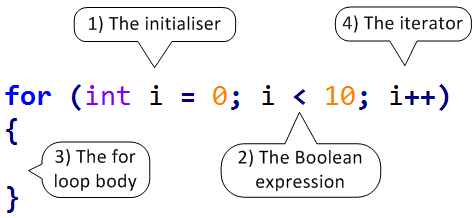
\includegraphics[width=0.6\textwidth]{c5.motif.for.01.png}
    \vspace{0.5em}
    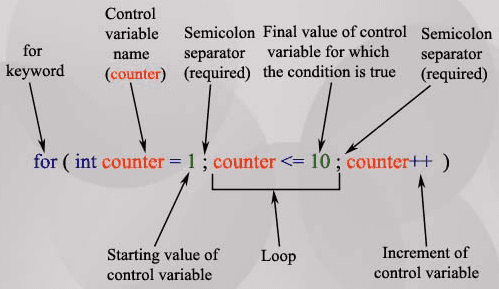
\includegraphics[width=0.6\textwidth]{c5.motif.for.02.png}
  \end{figure}
\end{frame}

\begin{frame}
  \frametitle{基序和循环 | 计数核苷酸 | 操作字符串 | \alert{for}}
  \begin{figure}
    \centering
    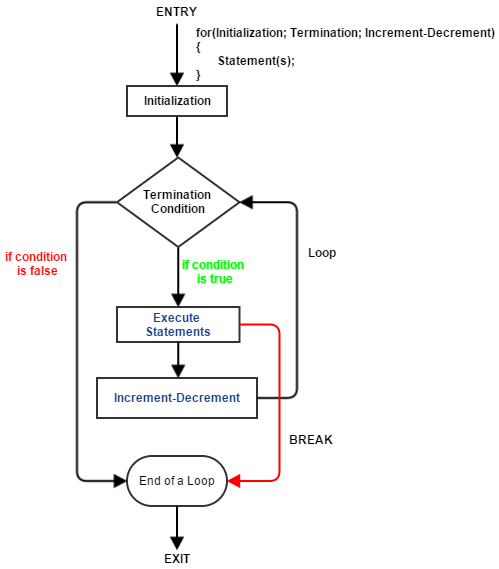
\includegraphics[width=0.56\textwidth]{c5.motif.for.flow.01.png}
  \end{figure}
\end{frame}

\begin{frame}
  \frametitle{基序和循环 | 计数核苷酸 | 操作字符串 | \alert{for}}
  \begin{figure}
    \centering
    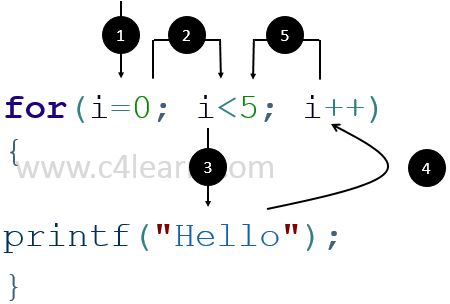
\includegraphics[width=0.5\textwidth]{c5.motif.for.flow.02.png}
    \vspace{0.5em}
    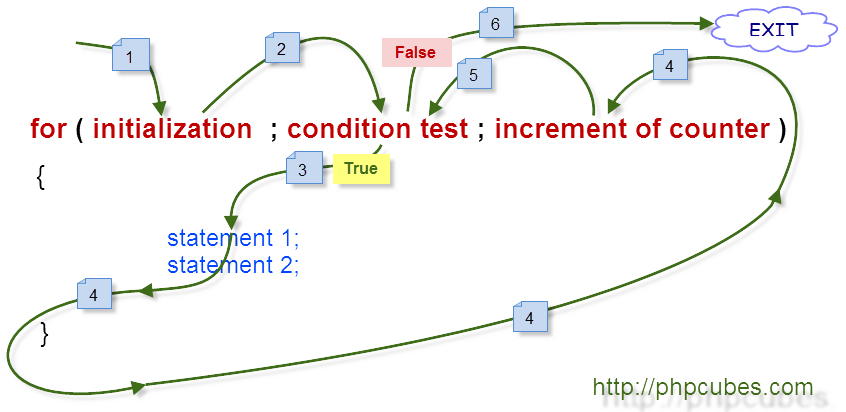
\includegraphics[width=0.6\textwidth]{c5.motif.for.flow.03.png}
  \end{figure}
\end{frame}

\begin{frame}[fragile]
  \frametitle{基序和循环 | 计数核苷酸 | 操作字符串 | \alert{for vs. while}}
\begin{lstlisting}
for ( $position = 0 ; $position < length $DNA ; ++$position ) {
  # the statements in the block
}
\end{lstlisting}
\pause
\begin{lstlisting}
# 等价的while循环
$position = 0;

while( $position < length $DNA  ) {
  # the same statements in the block, plus ...

  ++$position;
}
\end{lstlisting}
\end{frame}

\begin{frame}[fragile]
  \frametitle{基序和循环 | for循环 | 九九乘法表 | 正确 | for}
\begin{lstlisting}[basicstyle=\small\tt,numberstyle=\footnotesize]
#!/usr/bin/perl 

use strict;
use warnings;
use utf8;

for ( my $i = 1 ; $i <= 9 ; $i++ ) {
    for ( my $j = 1 ; $j <= $i ; $j++ ) {
        print "$j x $i = " . $i * $j;
        if ( $j == $i ) {
            print "\n";
        }
        else {
            print "\t";
        }
    }
}
\end{lstlisting}
\end{frame}

\begin{frame}[fragile]
  \frametitle{基序和循环 | for循环 | 九九乘法表 | 正确 | 等价while}
\begin{lstlisting}[basicstyle=\small\tt,numberstyle=\footnotesize]
#!/usr/bin/perl 
use strict; use warnings; use utf8;

my $i = 1;
while ( $i <= 9 ) {
    my $j = 1;
    while ( $j <= $i ) {
        print "$j x $i = " . $i * $j;
        if ( $j == $i ) {
            print "\n";
        }
        else {
            print "\t";
        }
        $j++;
    }
    $i++;
}
\end{lstlisting}
\end{frame}

\begin{frame}[fragile]
  \frametitle{基序和循环 | for循环 | 九九乘法表 | 错误 | for}
\begin{lstlisting}[basicstyle=\small\tt,numberstyle=\footnotesize]
#!/usr/bin/perl 

use strict;
use warnings;
use utf8;

# for的语法上没有错误!
# 但输出的不是九九乘法表!
for ( my $i = 1, my $j = 1 ; $i <= 9 && $j <= $i ; $i++, $j++ ) {
    print "$j x $i = " . $i * $j;
    if ( $j == $i ) {
        print "\n";
    }
    else {
        print "\t";
    }
}
\end{lstlisting}
\end{frame}

\begin{frame}[fragile]
  \frametitle{基序和循环 | for循环 | 九九乘法表 | 错误 | 等价while}
\begin{lstlisting}[basicstyle=\small\tt,numberstyle=\footnotesize]
#!/usr/bin/perl 
use strict; use warnings; use utf8;

my $i = 1;
my $j = 1;
while ( $i <= 9 ) {
    while ( $j <= $i ) {
        print "$j x $i = " . $i * $j;
        if ( $j == $i ) {
            print "\n";
        }
        else {
            print "\t";
        }
        $j++;
    }
    $i++;
}
\end{lstlisting}
\end{frame}


\begin{frame}[fragile]
  \frametitle{基序和循环 | 计数核苷酸 | 操作字符串 | \alert{索引}}
  \begin{block}{索引}
  \begin{itemize}
    \item 字符串:起始于0,最后一个字符的索引比字符串的长度小1
    \item 数组元素:第一个元素的索引为0,最后一个元素的索引为 \verb|scalar(@array)-1|,或者 \verb|@array-1|
  \end{itemize}
  \end{block}
  \pause
\begin{lstlisting}[language=]
字符串:ATGCGCAT
索引值:01234567
计数值:12345678

数组元素:A C G T G T A C
元素索引:0 1 2 3 4 5 6 7
元素计数:1 2 3 4 5 6 7 8
\end{lstlisting}
\end{frame}

\begin{frame}[fragile]
  \frametitle{基序和循环 | 计数核苷酸 | 操作字符串 | \alert{substr}}
\begin{lstlisting}
$base = substr($DNA, $position, 1);
\end{lstlisting}
\pause
\begin{block}{substr}
  \begin{itemize}
    \item 作用:获取位置索引为 \verb|$position|的那个碱基
    \item substr可以对字符串进行插入或者删除操作
    \item 第一个参数指定要操作的字符串
    \item 第二个参数指定要操作的位置索引(负值表示从字符串末尾开始)
    \item 第三个参数指定要操作的长度(负值表示字符串末尾剩余的字符数)
    \item 第四个参数指定要替换成的字符串
    \item substr vs. splice (操作字符串 vs. 操作数组)
      \begin{itemize}
        \item 语法
        \item 返回值
        \item 对原数组的“伤害”
      \end{itemize}
  \end{itemize}
\end{block}
\end{frame}

\begin{frame}[fragile]
  \frametitle{基序和循环 | 计数核苷酸 | 操作字符串 | \alert{substr}}
\begin{lstlisting}
my $s = "The black cat climbed the green tree";
my $color  = substr $s, 4, 5;      # black
my $middle = substr $s, 4, -11; # black cat climbed the
my $end    = substr $s, 14; # climbed the green tree
my $tail   = substr $s, -4; # tree
my $z      = substr $s, -4, 2;     # tr

my $r = substr $s, 14, 7, "jumped from";    # climbed
# $s is now "The black cat jumped from the green tree"
\end{lstlisting}
\end{frame}

\section{写入文件}
\begin{frame}[fragile]
  \frametitle{基序和循环 | \alert{写入文件}}
\begin{lstlisting}
# Also write the results to a file called "countbase"

$outputfile = "countbase";

unless ( open(COUNTBASE, ">$outputfile") ) {
  print "Cannot open file \"$outputfile\" to write to!!\n\n";
  exit;
}

print COUNTBASE "A=$a C=$c G=$g T=$t errors=$e\n";

close(COUNTBASE);
\end{lstlisting}
\end{frame}

\begin{frame}[fragile]
  \frametitle{基序和循环 | \alert{读写文件}}
\begin{lstlisting}[basicstyle=\small\tt]
# 读取文件
open my $FH, '<', $filename or die "$0 : failed to open input file '$filename' : $!\n";
... <$FH> ...
close $FH or warn "$0 : failed to close input file '$filename' : $!\n";

# 写入文件
open my $FH_OUT, '>', $fn_out or die "$0 : failed to open output file '$fn_out' : $!\n";
select $FH_OUT;
print "something...";
# OR: use $FH_OUT for every print
#print $FH_OUT "something...";
... 
close $FH_OUT or warn "$0 : failed to close output file '$fn_out' : $!\n";
\end{lstlisting}
\end{frame}

\begin{frame}[fragile]
  \frametitle{基序和循环 | 写入文件 | 计数核苷酸 | 程序5.7.1}
\begin{lstlisting}[firstnumber=1,basicstyle=\footnotesize\tt,numberstyle=\scriptsize]
#!/usr/bin/perl -w
# Example 5-7   Determining frequency of nucleotides, take 3

# Get the DNA sequence data
print "Please type the filename of the DNA sequence data: ";

$dna_filename = <STDIN>;

chomp $dna_filename;

# Does the file exist?
unless ( -e $dna_filename ) {

    print "File \"$dna_filename\" doesn\'t seem to exist!!\n";
    exit;
}
\end{lstlisting}
\end{frame}

\begin{frame}[fragile]
  \frametitle{基序和循环 | 写入文件 | 计数核苷酸 | 程序5.7.2}
\begin{lstlisting}[firstnumber=18,basicstyle=\small\tt]
# Can we open the file?
unless ( open( DNAFILE, $dna_filename ) ) {

    print "Cannot open file \"$dna_filename\"\n\n";
    exit;
}

@DNA = <DNAFILE>;

close DNAFILE;

$DNA = join( '', @DNA );

# Remove whitespace
$DNA =~ s/\s//g;
\end{lstlisting}
\end{frame}

\begin{frame}[fragile]
  \frametitle{基序和循环 | 写入文件 | 计数核苷酸 | 程序5.7.3}
\begin{lstlisting}[firstnumber=34]
# Initialize the counts.
# Notice that we can use scalar variables to hold numbers.
$a = 0;
$c = 0;
$g = 0;
$t = 0;
$e = 0;

# Use a regular expression "trick", and five while loops,
#  to find the counts of the four bases plus errors
\end{lstlisting}
\end{frame}

\begin{frame}[fragile]
  \frametitle{基序和循环 | 写入文件 | 计数核苷酸 | 程序5.7.4}
\begin{lstlisting}[firstnumber=44]
while ( $DNA =~ /a/ig )       { $a++ }
while ( $DNA =~ /c/ig )       { $c++ }
while ( $DNA =~ /g/ig )       { $g++ }
while ( $DNA =~ /t/ig )       { $t++ }
while ( $DNA =~ /[^acgt]/ig ) { $e++ }

print "A=$a C=$c G=$g T=$t errors=$e\n";
\end{lstlisting}
\end{frame}

\begin{frame}[fragile]
  \frametitle{基序和循环 | 写入文件 | 计数核苷酸 | 程序5.7.5}
\begin{lstlisting}[firstnumber=52,basicstyle=\small\tt]
# Also write the results to a file called "countbase"
$outputfile = "countbase";

unless ( open( COUNTBASE, ">$outputfile" ) ) {

    print "Cannot open file \"$outputfile\" to write to!!\n\n";
    exit;
}

print COUNTBASE "A=$a C=$c G=$g T=$t errors=$e\n";

close(COUNTBASE);

# exit the program
exit;
\end{lstlisting}
\end{frame}

\begin{frame}[fragile]
  \frametitle{基序和循环 | 写入文件 | 计数核苷酸 | 程序5.7 | 输出}
\begin{lstlisting}
Please type the filename of the DNA sequence data: small.dna
A=40 C=27 G=24 T=17 errors=1
\end{lstlisting}
\end{frame}

\begin{frame}[fragile]
  \frametitle{基序和循环 | 写入文件 | 计数核苷酸 | \alert{while循环}}
\begin{lstlisting}
while ( $dna =~ /a/ig ) { $a++ }
\end{lstlisting}
\pause
\begin{block}{while循环}
  \begin{itemize}
    \item i:不区分大小写(匹配a或者A)
    \item g:全局修饰符,匹配字符串中的所有a
    \item 没有g的话,如果字符串中有a,会陷入死循环
    \item 每一次匹配都会递增计数器(对字符串中的所有a进行计数)
  \end{itemize}
\end{block}
\end{frame}

\begin{frame}[fragile]
  \frametitle{基序和循环 | 写入文件 | 计数核苷酸 | \alert{tr}}
\begin{lstlisting}
$a = ($dna =~ tr/Aa//);
$c = ($dna =~ tr/Cc//);
$g = ($dna =~ tr/Gg//);
$t = ($dna =~ tr/Tt//);

$basecount = ($dna =~ tr/ACGTacgt//);
$nonbase = (length $dna) - $basecount;
\end{lstlisting}
\pause
\begin{block}{tr}
  \begin{itemize}
    \item tr函数返回它在字符串中找到的特定字符的数目
    \item 如果替换的字符集为空,原始的字符串不会发生改变
    \item 速度快,一个很好的字符计数器
    \item 需要同时指定大小写字母
    \item tr不接受字符集(没法直接对非碱基的字符进行计数)
  \end{itemize}
\end{block}
\end{frame}

\begin{frame}[fragile]
  \frametitle{基序和循环 | 写入文件 | 计数核苷酸 | \alert{length}}
\begin{lstlisting}
my $dna = "ACGT";
my $dna_len = length $dna;
print "$dna_len"; # 4

my @bases = ("A", "C", "G", "T");
my $bases_len = length @bases; # NOT USE!
print "$bases_len"; # 1
#Warning: length() used on @bases (did you mean "scalar(@bases)"?)
\end{lstlisting}
\pause
\vspace{-0.5em}
\begin{block}{length}
{\small
Returns the length in characters of the value of EXPR. If EXPR is omitted, returns the length of \verb|$_|. If EXPR is undefined, returns ``undef".\\
\vspace{0.2em}
This function cannot be used on an entire array or hash to find out how many elements these have. For that, use ``\alert{scalar @array}" and ``\alert{scalar keys \%hash}", respectively.
}
\end{block}
\end{frame}

\section{知识拓展}
\begin{frame}
  \frametitle{基序和循环 | 知识拓展 | 正则表达式 | \alert{基础}}
  \begin{figure}
    \centering
    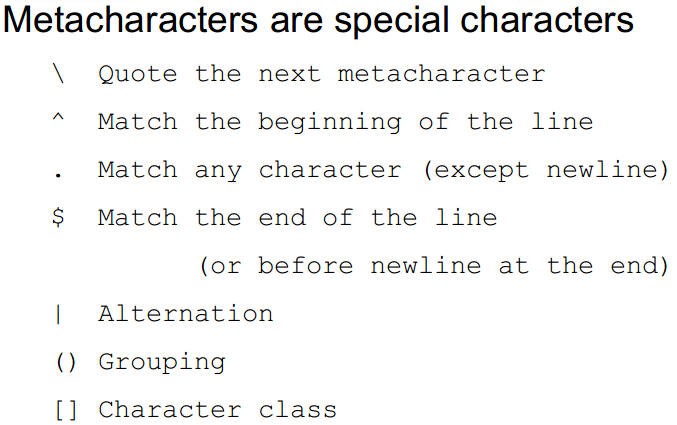
\includegraphics[width=0.35\textwidth]{c5.motif.re.basic.01.png}
    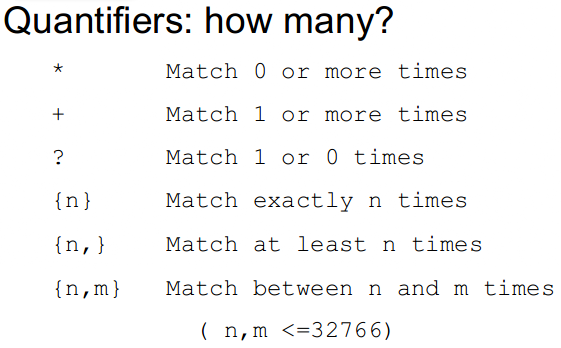
\includegraphics[width=0.32\textwidth]{c5.motif.re.basic.02.png}
    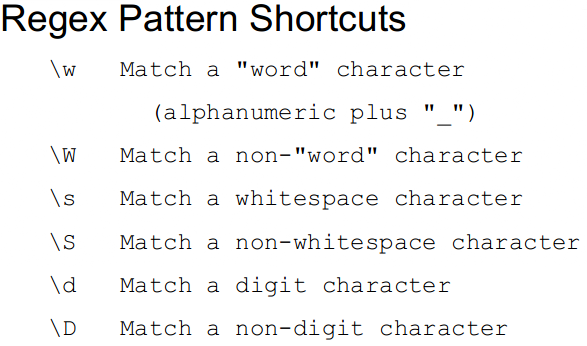
\includegraphics[width=0.33\textwidth]{c5.motif.re.basic.04.png}
    \vspace{0.5em}
    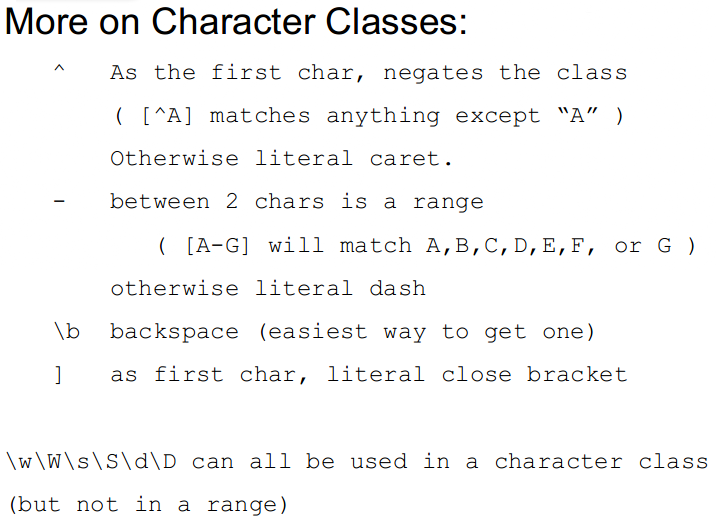
\includegraphics[width=0.36\textwidth]{c5.motif.re.basic.05.png}
    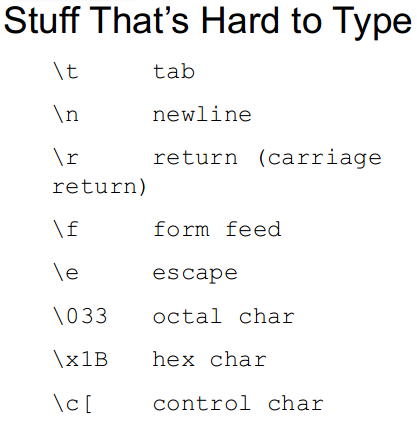
\includegraphics[width=0.22\textwidth]{c5.motif.re.basic.03.png}
    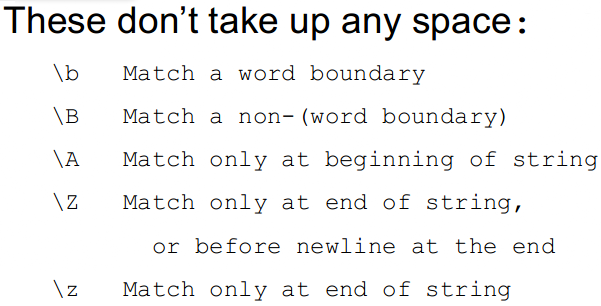
\includegraphics[width=0.35\textwidth]{c5.motif.re.basic.06.png}
  \end{figure}
\end{frame}

\begin{frame}
  \frametitle{基序和循环 | 知识拓展 | 正则表达式 | \alert{基础}}
  \begin{figure}
    \centering
    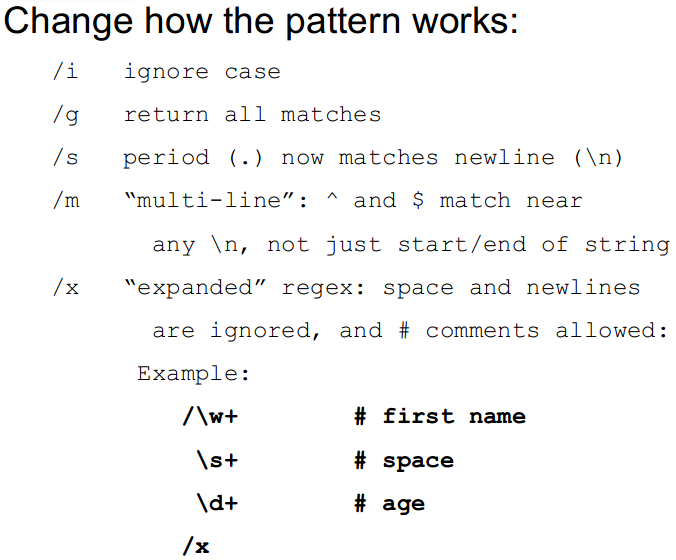
\includegraphics[width=0.7\textwidth]{c5.motif.re.basic.07.png}
  \end{figure}
\end{frame}

\begin{frame}
  \frametitle{基序和循环 | 知识拓展 | 正则表达式 | \alert{基础}}
  \begin{figure}
    \centering
    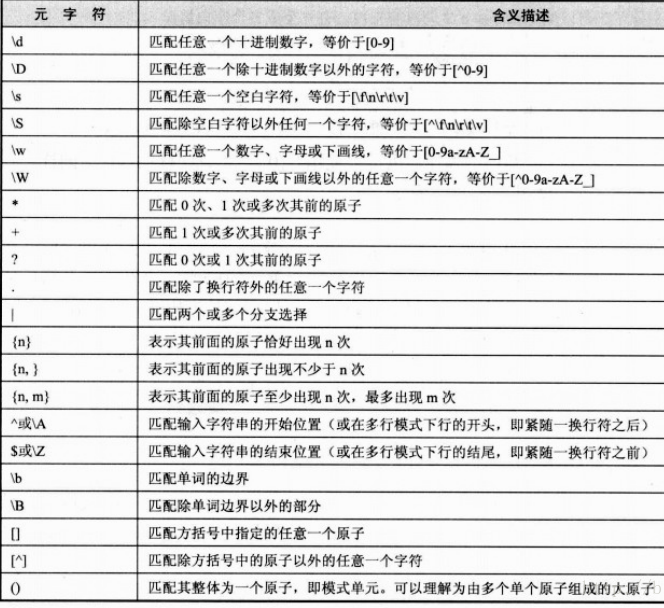
\includegraphics[width=0.7\textwidth]{c5.motif.re.meta.01.png}
  \end{figure}
\end{frame}

\begin{frame}
  \frametitle{基序和循环 | 知识拓展 | 正则表达式 | 总结}
  \begin{figure}
    \centering
    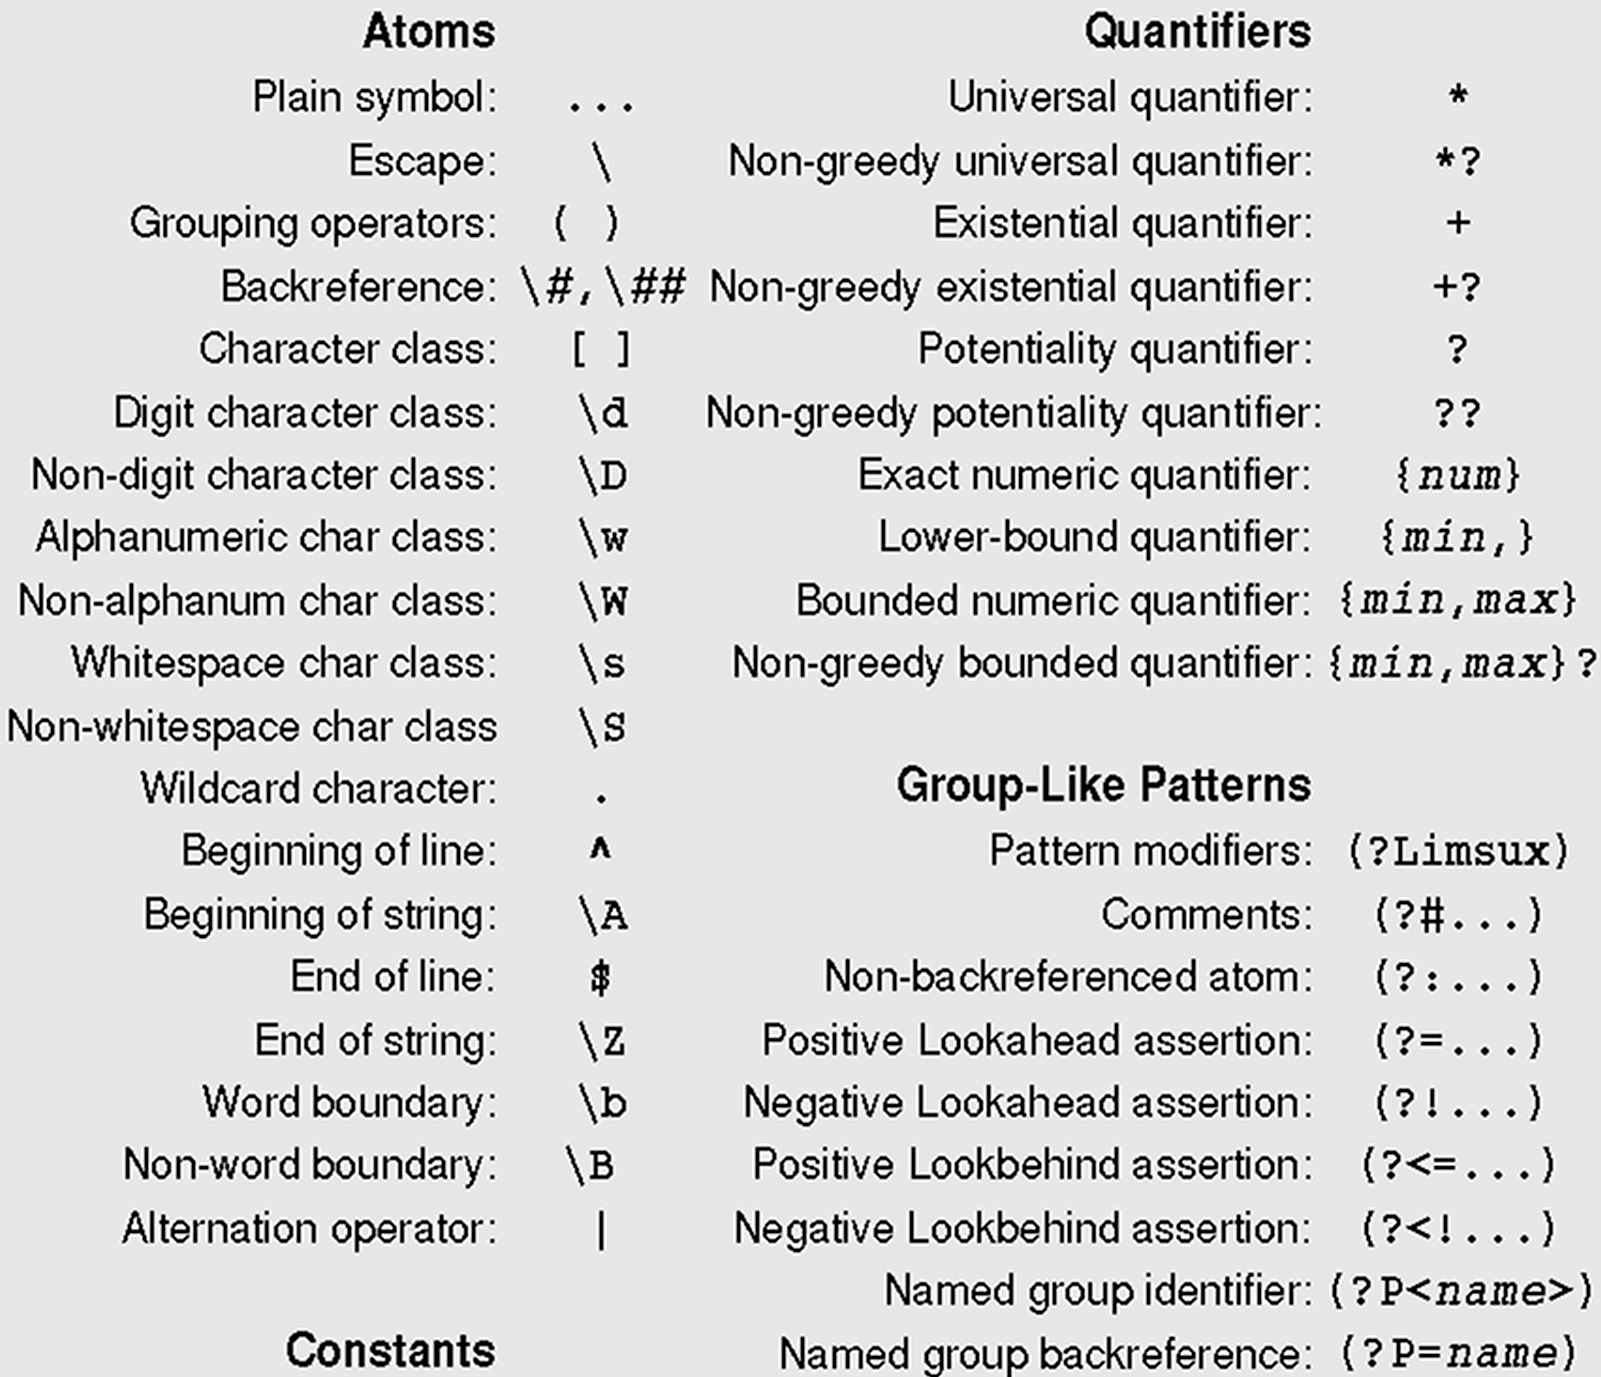
\includegraphics[width=0.75\textwidth]{c5.motif.re.01.png}
  \end{figure}
\end{frame}

\begin{frame}
  \frametitle{基序和循环 | 知识拓展 | 正则表达式 | 总结}
  \begin{figure}
    \centering
    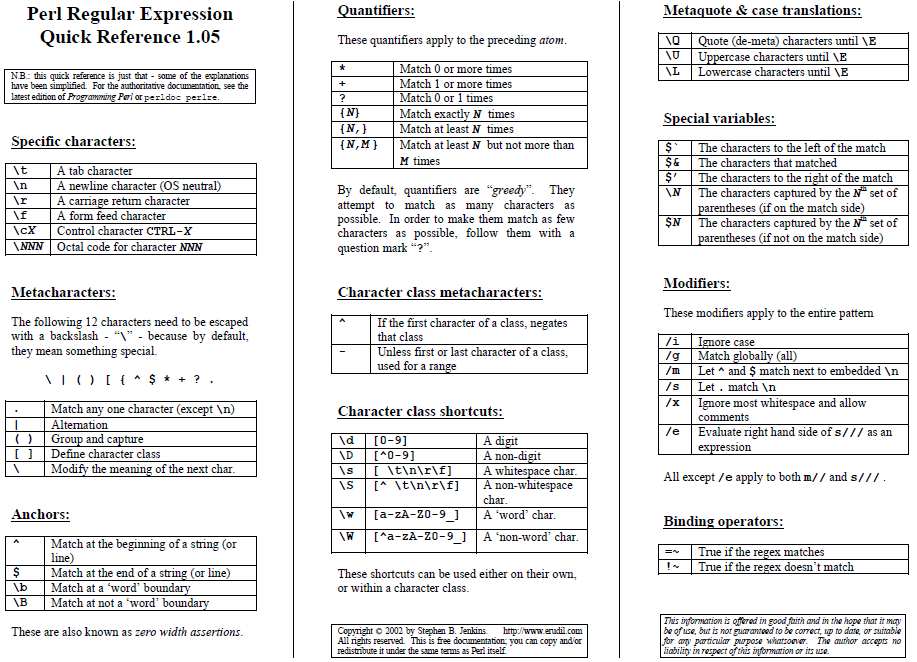
\includegraphics[width=0.9\textwidth]{c5.motif.re.02.png}
  \end{figure}
\end{frame}

\begin{frame}
  \frametitle{基序和循环 | 知识拓展 | 正则表达式 | 实例}
  \begin{figure}
    \centering
    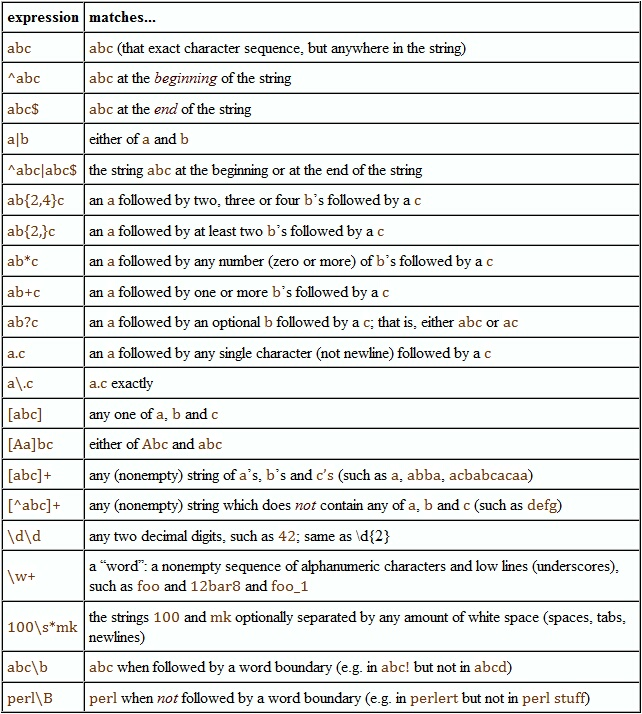
\includegraphics[width=0.58\textwidth]{c5.motif.re.example.01.jpg}
  \end{figure}
\end{frame}

\begin{frame}
  \frametitle{基序和循环 | 知识拓展 | 正则表达式 | 实例}
  \begin{figure}
    \centering
    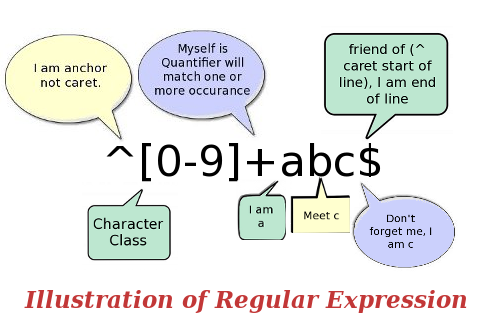
\includegraphics[width=0.45\textwidth]{c5.motif.re.example.02.png}
    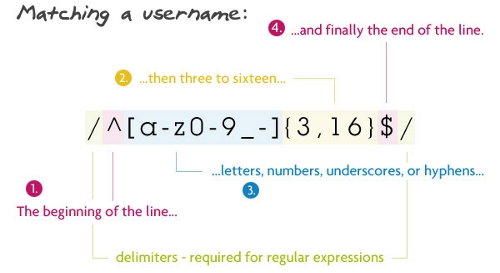
\includegraphics[width=0.53\textwidth]{c5.motif.re.example.03.jpg}
    \vspace{0.51em}
    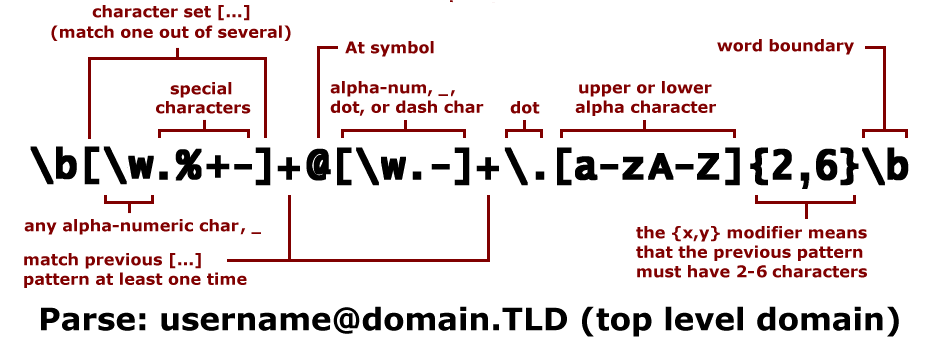
\includegraphics[width=0.85\textwidth]{c5.motif.re.example.04.png}
  \end{figure}
\end{frame}

\begin{frame}[fragile]
  \frametitle{基序和循环 | 知识拓展 | 正则表达式 | 模块}
  \begin{block}{Regexp::Common}
    Provide commonly requested regular expressions.
  \end{block}
  \vspace{-0.5em}
  \begin{lstlisting}[basicstyle=\scriptsize\tt]
use Regexp::Common;
while (<>) {
    /$RE{num}{real}/               and print q{a number};
    /$RE{quoted}/                  and print q{a ['"`] quoted string};
   m[$RE{delimited}{-delim=>'/'}]  and print q{a /.../ sequence};
    /$RE{balanced}{-parens=>'()'}/ and print q{balanced parentheses};
    /$RE{profanity}/               and print q{a #*@%-ing word};
}
\end{lstlisting}
  \vspace{-0.5em}
  \begin{block}{Regexp::Common::X}
    Regexp::Common::time, Regexp::Common::URI, Regexp::Common::Email::Address, ...
  \end{block}
\end{frame}

\begin{frame}
  \frametitle{基序和循环 | 知识拓展 | 正则表达式 | 应用}
  \begin{figure}
    \centering
    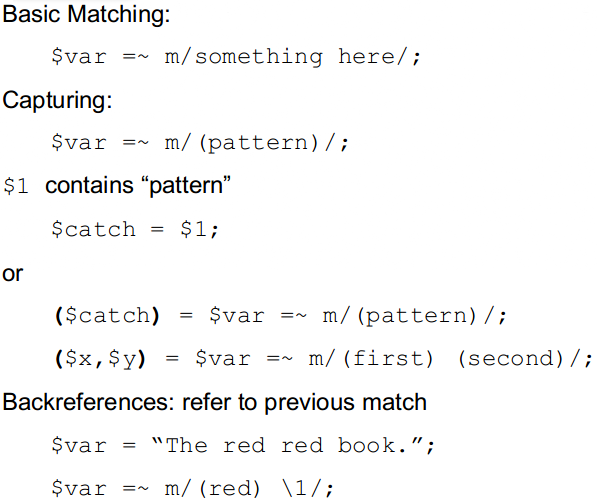
\includegraphics[width=0.45\textwidth]{c5.motif.re.use.01.png}\quad
    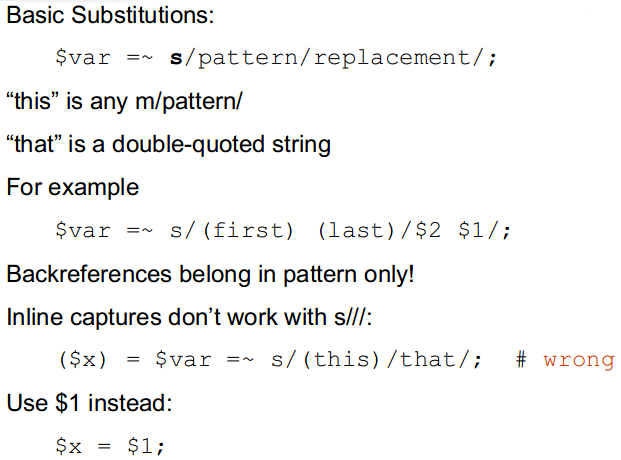
\includegraphics[width=0.5\textwidth]{c5.motif.re.use.02.png}
  \end{figure}
\end{frame}

\begin{frame}
  \frametitle{基序和循环 | 知识拓展 | 正则表达式 | 应用}
  \begin{figure}
    \centering
    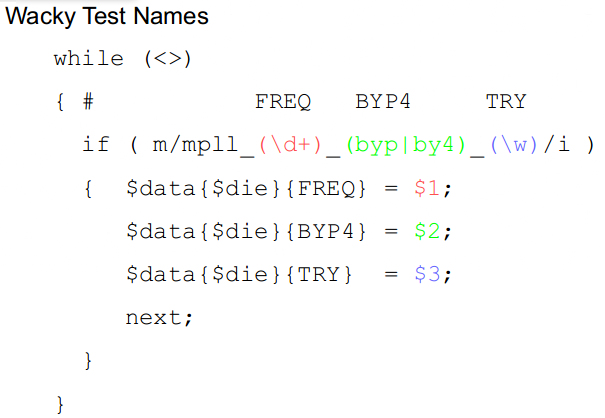
\includegraphics[width=0.8\textwidth]{c5.motif.re.use.03.png}
  \end{figure}
\end{frame}

\section{回顾与总结}
\subsection{总结}
\begin{frame}
  \frametitle{基序和循环 | 总结}
  \begin{block}{知识点}
    \begin{itemize}
      \item 流程控制的各种语句:条件判断,循环
      \item 文件交互:打开文件、读取数据、写入文件
      \item 标量和数组的转换:join,split
      \item 正则表达式:字符集,模式匹配
      \item 字符串操作:substr,tr
      \item 其他:真与假,获取键盘输入,变量初始化,智能化处理,特殊变量,递增,文件测试,索引
    \end{itemize}
  \end{block}
  \pause
  \begin{block}{技能}
    \begin{itemize}
      \item 能够熟练使用Perl语言中的各种流程控制语句
      \item 能够编写在DNA或者蛋白质序列中查找基序的程序
      \item 能够编写对DNA序列中的核苷酸进行计数的程序
    \end{itemize}
  \end{block}
\end{frame}

\subsection{思考题}
\begin{frame}
  \frametitle{基序和循环 | 思考题}
  \begin{enumerate}
    \item 总结Perl语言中进行流程控制的语句。
    \item 总结Perl语言中真与假的判断法则。
    \item 比较chomp和chop。
    \item 总结标量(字符串)和数组互转的方法。
    \item 总结正则表达式和模式匹配的使用。
    \item 如果不对变量初始化会怎样?
    \item 用实例说明Perl对数字和字符串的智能化处理。
    \item 总结substr和tr对字符串的处理。
  \end{enumerate}
\end{frame}

\begin{frame}
  \frametitle{下节预告}
  \begin{block}{问题}
 计数核苷酸的程序有好几个,但其实每个版本的大部分代码都是一样的,唯一改变的是计数碱基的部分。有没有办法能够比较方便地只改变计数碱基的部分呢? 
  \end{block}
  \begin{block}{回顾}
 shell编程中的函数(定义、调用、参数传递、作用域等)。 
  \end{block}
\end{frame}


\input{snippet/class_tail.tex}
